%\documentclass[man]{apa}
%\documentclass[doc]{article}{styles/apacls/apa}
%\documentclass{report}
%\documentclass[man]{styles/apacls/apa}

%\documentclass[11pt,twoside,a4paper]{article}
%\documentclass[11pt,twoside,a4paper]{book}
%\documentclass[11pt,twoside,a4paper,openright]{report}
\documentclass[11pt,oneside,a4paper,openright]{report}

\usepackage{mathptmx}       % selects Times Roman as basic font
\usepackage{helvet}         % selects Helvetica as sans-serif font
\usepackage{courier}        % selects Courier as typewriter font
\usepackage{type1cm}        % activate if the above 3 fonts are
                            % not available on your system
\usepackage[utf8]{inputenc}
\usepackage{textcomp}
\usepackage{makeidx}         % allows index generation
\usepackage{graphicx}        % standard LaTeX graphics tool
                             % when including figure files
\usepackage{multicol}        % used for the two-column index
\usepackage[bottom]{footmisc}% places footnotes at page bottom

\usepackage{verbatim}        % per comentaris multilinia
\usepackage[utf8]{inputenc} %permite escribir {\'a},{\'e},{\'u},{\'o},{\'\i} & {\~n} directamente
\usepackage[british]{babel}
\usepackage{csquotes}
\usepackage{amsmath, amsthm, amssymb}
\usepackage{enumerate}
\usepackage{algorithm2e}
\usepackage{pdfcomment}
%\usepackage[lined,boxed,commentsnumbered]{algorithm2e}


\begin{document}
\title{Coevolutionary strategies in MultiAgent systems. An approach using socionatural realistic environments.\\
\small{Master Thesis}}
\author{Alexis Torrano Mart\'inez}
\maketitle
\newpage

%\textwidth 6in \oddsidemargin 0.2in \evensidemargin -0.2in
%\textheight 9in \topmargin -0.75in \headheight 0mm \headsep 25mm

%\Large
%\addtolength{\hoffset}{-2cm}

\pagenumbering{roman}
\begin{abstract}
The aim of this master thesis is the development of a multiagent model for a simulation of two populations whose interactions are strongly influenced by a realistic landscape.\\
This research will be in line with Consolider-Simulpast (www.simulpast.es), an interdisciplinary project aimed to create simulations designed to be used in archaeological studies of human-environment interaction, decision-making processes and coevolutionary/competition behaviours of past societies.\\
The work plan will be focused on the development of first-stage models for two societies in the age of agriculture spreading surpasing the hunting and foraging way of living. The simulation will involve a climate engine for seasonality depending primarily on variable rainfall rate. Landscape information will be created from satellite image rasters. Constants, and variable relationship shall be modelled from measures and interviews with the experts. Data analysis tasks will be undertaken to validate the models and detect patterns in the archaeological record. Furthermore a comparison will be stablished between the classical simple models used in social simulation[1][2][8] and more advanced approaches.
\end{abstract}
\newpage 

\setcounter{tocdepth}{6}
\tableofcontents
\newpage 

\pagenumbering{arabic}
\chapter{Introduction}

\section{Description}

%Problem, Gujarat, Archeology (com al resum de la matri­cula).

\section{Motivation}

Simulation has been following an evolution in the models and paradigms applied to represent its target
systems. Dynamical systems, differential equations have been used and an overall simplification of the parts of the systems in the history of simulation to operate with the abstraction and simplification of the problems.
Mainly, reusing ideas from physical simulations, social sciences has modelled complex systems with dynamical
atomic entities that apply a simple set of centralized rules to move around the environment modelled. It was seen that due to the deeper details in human behaviour the question that could be solved and asked to that kind of models could not go very further as expected.

To solve non-linearity phenomena, heterogeneity, hysteresis\cite[p.571–597]{hysteresisDef} and other issues typical of complex systems, Agent Based Models(ABMs) where introduced to gain more insight of the modelled systems achieving good results. But under 
some conditions of very complex relationships between agents, highly specialized decission taking procedures
and issues in the environment led agents to need a sophysticated reasoning and problem solving capabilities
that are not specified and not yet introduced in ABMs coming from Social Sciences.

We have found an example of that situation in our case study located in Gujarat from Simulpast project. Our agents must interact with a regular but changing environment to get resources, plan its actions, coordinate with its group and compete with other groups in a \textbf{co-evolution} dynamic. Because we want to find out why the Gujarat HunterGatherer(HG) way of life lasted more than in other place of Earth in its competition against AgroPastoralist(AP), we need to embed the behaviours of the survival strategies used by these groups. A simply reactive agent cannot cope with short term plus long term decissions in that competitive environment. So the question stated as topic for this Master Thesis project is \textbf{``do we get better results in social sciences simulations adding deeper AI techniques to make richer the behaviour or decission making engines of the entities in the system?''}. As we understand ``better results``, the outcome from the use of AI should be a more sound validation of the model, a nearier match of modelled behaviours with the real ones, and clearer, richer and robust scientific conclusions.

In order to study such posibilities Sugarscape is a good framework to extend. Sugarscape is an artificial society developed by Joshua Epstein et al \cite{EpsteinAxtell}. where a number of inhabitants move to collect resources they need to live. Sugarscape models perception, lattice scanning in search of resources, sexual reproduction of the agents in the simulation, market relationships, immunology and spreading of diseases, and feature evolution. Epstein analises different experiments executed in the Sugarscape offering his conclusions and the dynamics emerging from the simulations. The results and conclusions will feed our AI experiments in order to make the comparisons of classical SugarScape agents vs AI agents, therefore, giving an answer to the topic of the Master Project.

\section{Simulation}

%brief description
%hi ha altres aplicacions de simulacio on no hi ha component temporal i no ho estic esmentant! MonteCarlo,etc...
Simulation is a discipline for performing virtual experiments in a computer. Computational techniques are used to build a model that represents your system. The dynamics of that system is codified in an algorithm that computes a calculus imitating the changes of state in the model, hence having a representation of that change along the time of the system modelled. Simulate is to play to ''what happens if...?'', and it is aimed to discover and explain the dynamics of a system to enhace or guide strategy development, decission taking, management, solving problems without analytical solutions or knowledge discovering and research. Although, we could get other positive benefits from it like theory checking or training through the inmersion in virtual worlds responding to our input.

% purpose, a priori, outcome, { deduction, induction, abduction(Alexis) } Axelrod's
% crec que els agradara, marketing, saborcillo de IA impregnant els racons
A simulation obeys some direction of experimentation, so a question must be set to drive the selection of features to model from the real system and give a direction to the modelling and the experiments design.These assumptions choice will prune the details not related to the questions to solve. It is not just for the sake of simplicity but for the practical reason that a model too near of the real system will be as hard as the original system to analyse.\\
Simulation, like deduction, starts with a set of those explicit assumptions. But unlike deduction, it does not prove theorems. Instead, a simulation generates data that can be analysed inductively. Unlike typical induction, however, the simulated data comes from a rigorously specified artificial experiment rather than direct measurement of the real world. While induction can be used to find patterns in data, and deduction can be used to find consequences of assumptions, simulation modelling can be used as an aid intuition and hypothesis validation tool. Also as space search mechanism for parameter tunning or optimization. This links with abductive processes.
%abduction
Just like in a tipical Sherlock Holmes case you pick the evidences, scenario for the experiment, and the common knowledge (the initial expert assumptions about the model). You enter in a refinement cycle where you test hypothesis and readjust them to discover the theory, the ``plot'', the explanation of what is happening. Following the abductive reasoning schema one looks for the hypothesis that would best explain the relevant evidence \cite{Axelrod2003}.\\
%% no anava errat amb l'abduccio! :D

%--: simulation, results, validation and statement of your inital hypothesis and question...
%--: simulation connected to abduction
% connect abduction with the simulation lifecycle 

Social simulation is a research field that applies computational methods to study issues in the social sciences. The issues explored include problems in psychology, sociology, political science, economics, anthropology, geography, archaeology and linguistics \cite{TakahashiSallachRouchier2007}.\\
Social simulation aims to cross the gap between the descriptive approach used in the social sciences and the formal approach used in the hard sciences, by moving the focus on the processes/mechanisms/behaviors that build the social reality.\\
In social simulation, computers supports human reasoning activities by executing these mechanisms. This field explores the simulation of societies as complex non-linear systems, which are difficult to study with classical mathematical equation-based models.
%reducibility 
Most of the times, studying complex systems implies to cope with non reducibility. One of the examples is Gravitational Dynamics. If our assumption is the use of Newton's mechanics, we can predict the state at any time or not, depending on the scenario. For a one dimension world you can predict the state at time $t_n$ from the initial state $t_0$ without computing all the preceding ones. For two and more dimensions you can only compute directly state $t_n$ if less the three bodies are implied. So in a real environment of many bodies in a 3D world you need to compute all the states from the initial to the one you consider as the last one. The system is non analytically reducible and you are forced to apply simulation to visit all the states and develop the behaviour of the model. It happens in most of the complex systems models, they have a nonlinear specification. Nonlinear models do not have a simple or computational reasonable analytical solution. 
% ( Classical Physics formulae used are non linear, acceleration is a quadratic factor in position <-- revisa aquesta fantasmada ) 

%emergence
Other of the main issues in complex systems simulation is emergence. While the initial assumptions may be simple, the consequences may not be at all obvious. The large-scale effects of locally interacting entities are called "emergent properties" of the system. Emergent properties are often surprising because it can be hard to anticipate the full consequences of even simple forms of interaction. 

%why simulation? because I need this non deducible emergence and the non deducible end state
There are some models, however, in which emergent properties can be formally deduced. Good examples include the neo-classical economic models in which rational agents operating under powerful assumptions about the availability of information and the capability to optimize can achieve an efficient reallocation of resources among themselves through costless trading. But when the agents use \textbf{adaptive} rather than optimizing strategies, deducing the consequences is often impossible; simulation becomes necessary.
% i ara estic preparat per conectar amb Social Science Simulation : reducibility + emergence forces to use simulation in S.S.

% Applying Simulation in the framework of Social Sciences to approach to the hypothesis of Simulpast targets, in concrete, about the case study from Gujarat, CS1.
%
%simulacio de sistemes complexes : f\'isica de particules, mercats, ... ecologia i... social sciences...
%
%n-body problem
%  2 body : formula
%  n body in 2D  : formula
%  n>2 body in 3D : simulation, non reducible
%   gravitation, electrostatics : input=initial position, output=end position, classical physics formulae: non linear!!!
%   acceleration is a quadratic factor in position!!!
%
%mes endevant cal caracteritzar la simulació : deterministic/stochastic, static/dynamic, open/closed, %linear/nonlinear, hysteressis, stable/unstable,
%stationary stage, emulation/monteCarlo/traceDriven/DiscreteEvent/DiscreteUnitTimeStep
%
%
%
%
\section{Question} 

% trobo a faltar m\'es xixa te\`orica, aix\`o s'hauria de semblar m\'es a un cap\'itol del Norvig.
In classical simulation approaches, specifically in the branch of Social Simulation, active entities which model human actors are designed with very simple behaviour engines. The classical hypothesis is that a complex mind for entities in the simulation are not that needed and maybe even could lead to difficult analysis of final results of the simulations (too daring statement?). 

Our statement is that, on the contrary, the mind engine of a simulation entity should not be bounded to that limit but special attention must be paid to give any necessary sofistication to give the entity a correct behaviour, real enough, sensible to the changes in the environment and competent to solve the issues that will have to solve along its lifetime in the system. Even more, we think that this entities' capability to respond with complex behaviours is the core that roots the modelling granularity needed to catch the essential of the social systems that we want to model.
%TODO ( a l'apartat de ABMs ho tornem a dir però afegint que cal adaptabilitat, resposta no lineal, aprenentatge depenent del temps, histeresis,...).\\
%( i aixo motivaria els ABMs) 
Applying such premises we will explore the possibility to give or enhance decission making, problem solving
capabilities to the entities with the aim to get more accurate simulations and realistic models with higher matching against our job hypothesis and premises. We will take the framework of ABMs to integrate the AI techniques in a decission making schema of action-response dynamics sensible to a modelled world.

%% ABM -> Decentralization of Decision-Making

%%exposicio mes detallada dels punts febles que creus que trobaràs als simple agents (i a les conclusions 
%% d'AI-Sugarscape se't confirma 
%% i d'altres outcomes)
\begin{enumerate}
 \item \indent \textbf{Do AI techniques contribute to better simulation results?}
 \item \indent \textbf{Classic Simple Agent approach vs Rich Agents}
 \item \indent \textbf{Did Gujarat extreme enviromental conditions delayed the HG disappearence?}
\end{enumerate}

\newpage 




\chapter{Methodology}

% on poso els steps del modelling procedure????
% specificacion --> expert's knowledge --> modelling --> prototipe --> { accept model | go to a previous state }
% revisiting early stages to refine models : toy model --> reviewing your assumptions about the main purpose
% interviews and ecotono meetings to motivate and help knowledge extraction
% ecotono modellings as a means to gain insight of the problem and the system, inspirational ideas.


\section{Intro}

%% metode = modelling\\
%% tecnica en ciencies socials = ABMs \\
%% afegir capitol llibre Rub+Cris\\

%que es modelling en ciencies socials 

% ATM mini intro

%hi ha un problema, analitzar-lo per solventar-ho, rational activity -> models

Modelling is a widely extended methodology to answer the kind of questions we set out. It comes from the natural observation of the world and the curiosity or need to reproduce it.\\
The modelling activity determines aspects of the world to include or exclude from the details that
will conform an abstraction of the world that will allow work the answers \cite{Robinson2008}.
%TODO multiple ref resuse : split in chapters/paragraphs

%% Robinson2008
%% In broad terms, conceptual modelling is the process of ab-
%% stracting a model from the real world. The modeller is pre-
%% sented with a problem situation that is amenable to simula-
%% tion modelling and then has to determine what aspects of
%% the real world to include, and exclude, from the model, and
%% at what level of detail to model each aspect. These deci-
%% sions should generally be a joint agreement between the
%% modeller and the problem owners i.e. the stakeholders who
%% require the model to aid decision-making.

%% >>> conceptual modelling is the process of ab-
%% stracting a model from the real world.

%% >>>then has to determine what aspects of
%% the real world to include, and exclude, from the model, and
%% at what level of detail to model each aspect.

%% \cite{Robinson2008}

%%Pidd
%% Models are convenient worlds. They are artificial worlds that have been deliberately 
%% created to help with understanding the possible consequences of particular actions. 
%% They are part of a process of ‘‘reflection before action’’ (Boothroyd, 1978). The 
%% models may be quantitative or qualitative, but in any case they will be simplified 
%% abstractions of the system of interest.

%% >>>> They are artificial worlds that have been deliberately 
%% created to help with understanding the possible consequences of particular actions.

%% >>>> The models may be quantitative or qualitative, but in any case they will be simplified 
%% abstractions of the system of interest.

%% \cite{Pidd2003}

Modelling will be our framework for communication between archeologists' and sociologists' knowledge and their conceptualizations with our formal representations from computer science practices( simulation, algorithms, AI ).
The reason is that it is a procedure that will help to communicate the \textbf{discursive} nature of Social Sciences with the formal structures from Computer Science. The enginering of model development will allow us to reach a connection from experts' knowledge to a model that comprises the set of detail clearing out the ambiguity that language could filtrate. Also, modelling will help set a picture of the system without inconsistencies, with each fact sound, coherent and consistent from the logical point of view with the whole.

\section{Why model}
% ATM, que es modelar? i com es modela?
%
The modelling process consists in identifying separable entities, processes, relationships and any rellevant information related to the question to solve and the domain of study. 
This abstraction exercise yields an external and explicit representation of part of reality as seen by the
people who wish to understand, to change, to manage or to control that part of reality \cite{Pidd2003}.\\
Indeed just thinking about something implies an unconscious projection of our mental frame hence producing a set of concepts and relationships that give birth to a model. The missed step is that it was not made explicit through some formal representation. A model is a logical and conceptual prototipe.\\
As Epstein \cite[p.1]{Epstein2008} says \textit{''Anyone who ventures a projection, or imagines how a social dynamic, epidemic, war, or migration would unfold is running some model``}.\\
Modelling is an introspection exercise where you take into account the domain to elaborate a \textbf{formal} representation of the conceptualizations you develop around the problem. Mainly, it will have to do with mathematical expressions from calculus or algebra and logics. That is called \textbf{conceptual modelling}. This phase comprises the development of a relevant simplification, which must be complete according to the phenomena that inspires the question. Anything left out will change the outcome of the simulation, and non-relevant added items will produce noise that will difficult posterior analisys. All the involved facts must be correctly well grounded taking into account that any unneeded compound in the model will also be added to the scientific and mathematic justification, adding good-for-nothing effort.\pdfcomment{ATM:Epstein buscant lloc concret on ho diu}\\
%%TODO ''good-for-nothing'' : busca paragraf on Epstein diu aixo  
%TODO reuse cite; split in chapter/paragraph?
For instance, lets consider modelling the dynamics of a restaurant to find an optimum allocation of waiters between interior and terrace tables and their serving policy, so it could be minimized the hired waiters while lowering the waiting time of clients. Variables like client arrival rate, kitchen serving time, number of interior tables, number of terrace tables are reasonable parts of the system to add to the simplification. The colour of the courtains, the outfit of the waiters most probably will not account for the stated optimization objective. Someone could argue about the topology of the tables whether it should be added or not to the model. But if the objective is to model the system to analyze the survival rate when there is a fire and people must exit from the building as soon as possible, table and furniture topology is an unquestionable variable.\\
This kind of criteria should lead to a preference for simpler models. There are many reasons which force to design consciously with this premise. More complex models require harder effort to work their credibility, verification\pdfcomment{XR:Verification or validation?}\\ \pdfcomment{ATM:Verification->Comprovar que el model esta ben implementat.Model simple:dificil.Model complexe:+dificil} for the correct implementation of the conceptual model, and from the formal point of view, validation of the model and the scientific conclusions. Considering the system conceptualization and formalization, a more complex model is more open to criticism for the objective or subjective choice of features and modelling decisions. Why the present features were chosen and the missing ones were left out? why one expert point of view, and not other one? Also, as Robinson \cite{Robinson2008} states, simple models have many advantages, such as they are faster, require less data, are more flexible. But the crucial point is if we better understand them we can better interpret their results. Constituents in models interact each other following the relationships established by the modellers. This produces a network or causality chain that is responsible of the state changes of the model along the simulation. These chains must be inspected to find the origin of the phenomena exhibited in the simulation. As we want to understand a system we must reconstruct the processes that lead to the outcome we observe or check against our assumptions or real world events. If we are designing models where constituents are grouped to conform more complicated constituents, if we design the model to exploit emergent phenomena, analisys of the outcome and the causality chain reconstruction will be a very difficult task to disentangle \cite[p.31]{Premo2010}\label{myPremo_simplicity}. Simplicity is a must. Besides, we are not aiming at a very rich and complex model that matches its outcomes almost perfectly with some referential real data. As it is explained below we have preference for a model that makes easier the task to explore social processes to answer and propose arising questions. We must find the causal conection between experimental parameters and model dynamics, which parameters under which diferent initial conditions make the system behave differently and say why.
Another concern is that detail and granularity choice are attached to the overall direction that takes the construction of the model in terms of structure. At this point it is interesting to mention how does a model can be grown.\\
%
According to Oppenheim's and Putnam's\cite[p.1-2]{McGivernAndRueger}\cite{Unity_of_Science}, theories describe their domain as a corpus of interelated concepts where the pieces of knowledge are connected with mathematical, hierarchical, structural and logical relationships, to enumerate some. The hierarchical relationships induce a multilayered organization of knowledge, sometimes called ontology\footnote{We are not talking about knowledge representation from A.I.}. The hierarchy of layers is related to the level of the abstraction of the contained concepts, going from concrete concepts to abstract ones that contain or subsume the former. Also, the composition relationship makes arise a hierarchy of layers. For instance, in social sciences, considering individuals which are part of families, families which are part of social groups, and groups which conform a society. 

%%TODO poso el següent ??
%% granularity, precission, level of detail,...
%% hunt, prey pack, 4 levels of detail
%% 1.- number of preys
%% 2.- number + probab distrib along the landscape
%% 3.- number + gas dynamics
%% 4.- swarm of agents (introduce lower level, from group to individual)

%% hierarchy relationships -> abstraction -> contain, subsumption, isA...

%% hierarchy relationships -> composition : cargol -> engranatge -> motor -> cotxe
%% hierarchy relationships -> composition : individual -> family -> social group-> society

% end arrange

%TODO
	%what is an atomic concept for you will be an abstract or compound concept for another theory.
	%what is a top abstract concept for you will be a concrete concept for another theory
%

Usually, modelling methodology takes either the top, bottom or a midle layer to crystalize the model following the hierarchy in a direction towards the higher concepts or the deeper ones. An ascending crystalization from simpler to more complex is called \textbf{bottom-up} and the inverse direction is known as \textbf{top-down}. Crystalization could begin in a midle layer and stop before arriving a top or bottom bound layer.\\ 
For instance, some simulation would consider a necessity to model individual persons with agents taking decission at that scale. Other simulations would model households with the decission process without having to consider individual persons. Once set this issue, the modelization could keep considering more abstract structures like families or tribes as a composition of households and stop here instead of continuing adding villages or countries to the model.\\ 
The point is that the range of concepts that you choose to include in the model is related to the level of detail you want apply to descrive the constituents of the model. The simplest chosen concepts that merge as constituents of other complex constituents and phenomena mark the granularity of your model. 

% 
% 1 .- set range of concepts, move either top-down or bott-up
% 2.- concensus for one bound (bott or top) and begin to grow till you see it is enough
%

%George Box
Although good modelling of the parts could be accomplished accurately lefting out the non-relevant entities and phenomena, let's remember the famous quote of George Box, ``essentially, all models are wrong, but some are useful'' \cite[p.2]{Box1979}.
\pdfcomment{has de dir d'on surt la cita}\\ \pdfcomment{ATM:done}

% multidiscpl ATM

By the way, it can also happen that the modelization requires go further the bound. For instance, consider we are modelling a society to see the emergence of some differentiated groups, in our project, hunters, gatherers, agropastoralists \pdfcomment{differentiated groups? Vols dir different cultural identities, potser? Perquè no dius de quin tipus de grups parles.}\\ \pdfcomment{ATM:done. No deia els grups concrets perque volia anar a parar a la multidisciplinarity que era el target del paragraf}. We could model towns, neighbourhoods, go down to families and then arrive to the person. Maybe we would like to characterize persons with some inner traits related to their personality as anxiety, generosity, aggressiveness, cooperation aptitude. Now we are entering in a layer belonging to psychology sciences, we have surpassed the bottom conceptualization in sociology. If we go further we could arrive to the brain structures entering the field of neurology. We could continue to mollecules, biochemistry, and so on and so forth\cite[p.56]{MWilliams1999}.\\
Trespassing these borders and needing the help of experts able to manage and modelize the concepts will be the motivation for multidisciplinarity. 

%TODO must I put it in Gujarat chapter? In our Gujarat project we are experiencing interaction between different disciplines of social sciences : anthropology, archeology, and sociology. Each one of these branches has its own terminology, target problems and argue their discurse with different structures.\\

Besides having to cope with implicit ambiguity in each discursive knowledge (as said before, Social Sciences usually represent their knowledge in discursive texts using natural language), all these branches must cooperate in a common framework connecting the different used conceptualizations. Some branches can organize their knowledge in concepts of entities, other use processes or actions, for instance. We cannot collapse this frameworks directly in a formal model. The modelling process will ellicite this structures and will match them with the mathematical tools offered by the chosen paradigm( lets say Dynamical System Theory, Agent Based Models, Petri Nets ). We will translate the conceptualizations to a common language that will connect the formalizations in a whole, the \textbf{conceptual framework}.\\
Modelling will help to find a consensus for expressing the concepts and properties, will help to ellicite knowledge, arrange ambiguities, detect common points. It will allow as to embed the needed rigor to work under the same framework to make every part work together. Modelling shall be an exercise of shared development that can approach positions and circle a communication problem to solve the issues that will arise.
% posar les 2 figures de multidiscp modelling

%%TODO
%ellicitation 
%posar l'exercici de comprensio entre BSC - IMF, elicitation, ecotonos...? o deixar-ho per capitols posteriors?


\section{Modelling in social sciences}
\label{sec:modelsinSC}

%%TODO afegeixo quelcom com aixo?
%% com la fisica ha tingut la seva matematica molt avancada, les CienSocials
%% reusen molt de les metafores i analogies que fa la fi­sica de la matematica
%% als seus sistemes -> buscar models fi­sics que no son sound ( busca publicacions,
%% analitza model de Fort, critica'l) -> processos amb cultura/expansio d'idees o espai de temps
%% diferents no es poden modelitzar amb fi­sica. 

%%%% content

Social science refers to the academic disciplines concerned with society and human behavior\cite[p.7,chap.3]{MWilliams1999}.
\\
We will take the point of view where the study of society or social groups considers its target as an adaptative ecosystem of people with interaction, other living entities, environmental conditions or environmental dynamics, information exchange and the mutual adaptative changes induced between the actors, co-evolution \cite[p.4]{PerezAndBatten2006}.\\
\pdfcomment{aviam...només són alguns investigadors que consideren la societat com un sistema adaptatiu. La inmensa majoria no ho fa, et caldria refer això. D'altra banda, si cites un llibre has de dir la pàgina o pàgines a les que t'estàs referint}
\\
\pdfcomment{ATM: ?`trec la frase que diu que prenem el punt de vista d'alguns investigadors que consideren la 
societat com un sistema adaptatiu? L'adaptabilitat va quedant esmentada sobretot en parlar d'agents, de sistemes
complexes que exhibeixen adaptabilitat... Aixo ja impregna el nostre punt de vista,no? Es redundant tenir aquesta frase? per altra banda sobretot, l'objectiu d'aquests primers paragrafs es il.lustrar els items o issues a tenir
en compte quan modeles sistemes socials. Aquests items surten esmentats a la ``definicio`` de ciencia social.Aixo
motiva que diguis ''ei,aquests ingredients son els susceptibles de posar-los a un model``, la pedra angular per decidir
l'aspecte o l'estrategia del model... i aixo fa portar a la proposta d'agents com a paradigma que va molt be
per cobrir aquests issues... Per aixo, m'es mes important parlar de persones, grups socials, interaccions que no
pas esmentar al principi sistemes adaptatitius; trobant-ho interessant de dir, no es prioritari en aquest punt.}
 
%modelling targets/items, 
Modelling societies implies being aware of constituents identified by the social theories. Interacting entities form a society. Such entities are observed and abstracted from identifiable individuals, people, and activity units, for instance families, neighbourhoods or job partners, composed also of the same individuals. An individual leaves a trace of participations and interactions in the society through social processes. Such activities occur with other individuals, with some activity units or through them. Populations of individuals flow through the social structures, selectively participating and differentially performing \cite[p.8]{GordonBurt2010}. 
Ordinary living involves a participation of people in the social activities of family, leisure and holidays, shopping, work and travel. These activities within units are structured by relationships and choices, rules, rituals and randomness. Ordinary living also involves the participation of cultural ideas and artefacts in social activities.
\pdfcomment{Cal lligar millor aquest raonament}
\\ 
\pdfcomment{ATM:estic enumerant elements a modelar, els fenomens que han detectat les social sciences, per a saber quins elements son susceptibles d'incloure's a un model.On tinc l'error? em perdo}

Social sciences seek to understand not only how individuals behave under the social influence, but also how the interaction of 
many individuals leads to large-scale outcomes and global phenomena \cite[p.9]{GordonBurt2010}.\\ 
Modelization will be the construction of an \textbf{analogy} between these constituents and processes identified by social sciences as elements, procedures, terms or expressions in some \textbf{representation language} that allows to manipulate and reason about them.\\  
The main observed issues, individuals, units, processes or actions, flow and dynamics within units, are the frontline of the 
modelization aspects and motivation for the different paradigms appeared or adapted to solve the modelling objectives. New 
knowledge to infer from this identified phenomena will be the \textbf{descriptive} statement of observed behaviour, quantitative 
empirical \textbf{generalisations}, construction or assesment of \textbf{theories} and \textbf{prediction} models \cite[p.9-53]{Coleman1964}.


\begin{figure}[h]
\centering
\setlength\fboxsep{0pt}
\setlength\fboxrule{0.5pt}
\fbox{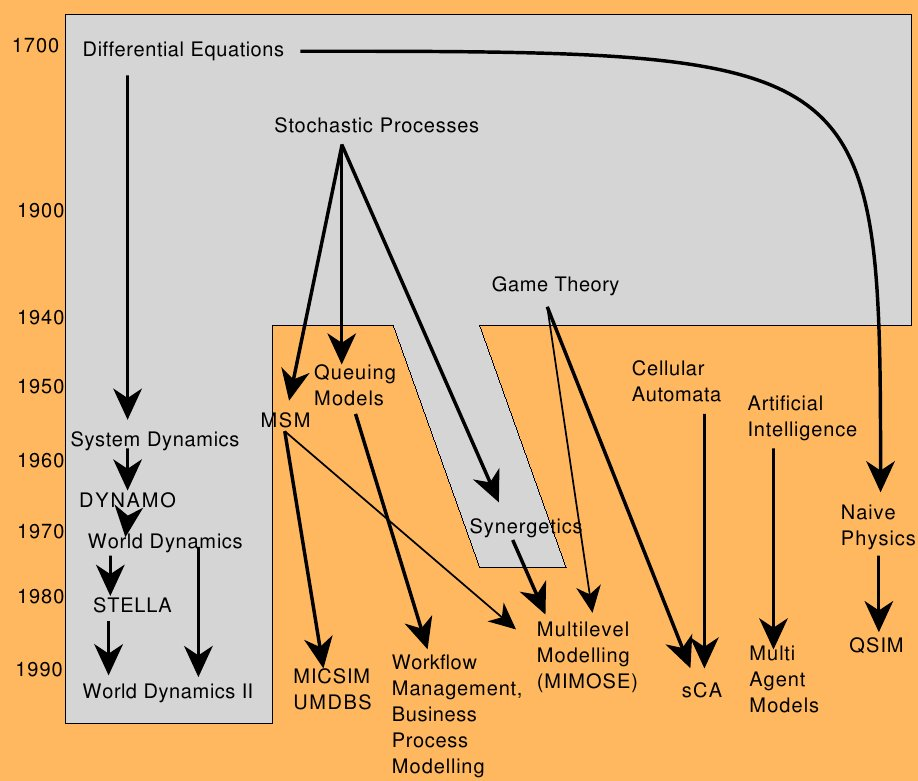
\includegraphics[width=120mm,keepaspectratio=true]{figures/Gilbert_pg21.jpg}}
\caption{The development of the first approaches to simulation in the social sciences (after Troitzsch \cite{GilbertTroitzsch})}
%by Gilbert \cite{GilbertTroitzsch}}
\label{fig:SimAppGilbTro}
\end{figure}

%possible paradigms. TOASK : Explico mes que son sistemes dinamics i la resta d'opcions?????

The first paradigms to model social processes were borrowed from the fields of physics, operations research, and economics. The first social concepts considered were those related to social units or subgroups and large processes. Also, due to the main use of dynamical systems and differential equations, social phenomena was modelled as a flow between different containers that represent groups or state of individuals.\\

\begin{figure}[h]
\centering
\setlength\fboxsep{0pt}
\setlength\fboxrule{0.5pt}
\fbox{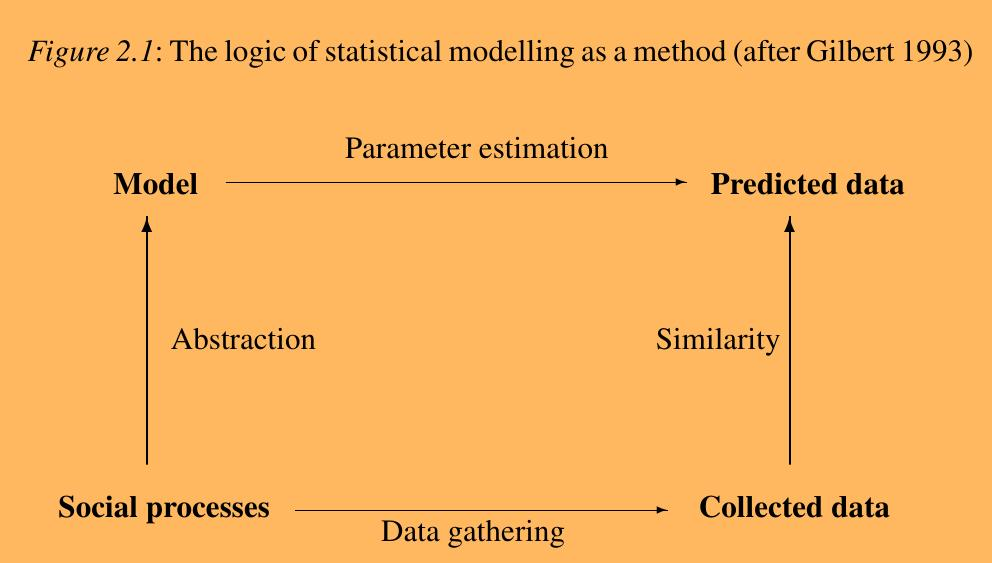
\includegraphics[width=120mm,keepaspectratio=true]{figures/statisticalModelling1.jpg}}
\caption{The logic of statistical modelling (after Gilbert 1993)\cite{GilbertTroitzsch}}
%by Gilbert \cite{GilbertTroitzsch}}
\label{fig:SimStatMod}
\end{figure}

Richer representations to cope with reality led to nonlinear specifications and the introduction of heterogeneity present in social systems making them hard to represent or analitically unsolvable, hence, the following years saw the spreading of \textbf{simulation techniques}, first AI aproximations, cellular automatas and Petri's networks that allowed a finer granularity going from the top abstract groupings infered in social theories to the individual entities\cite[chap.1,p.6-9]{GilbertTroitzsch}. 
%%TODO \cite{historic reference}


Gradually social modelling began to approach computational sciences keeping its connections to mathematics and statistics. Programming languages are more expressive, less abstract than most mathematical techniques. Programs deal more easily with parallel processes and processes without a well-defined order of actions compared to math equations. There is a quite long experience on studying programs and their properties from Algorithmics, Soft Engineering, and Operating Systems. The enginering of big models benefits from these branches endowing them with the desirable properties of modularity, extendibility, the experience of combining programs to grow huge program systems, error detection and maintenance, to mention some \cite{TaberAndTimpone1996}.

\begin{figure}[h]
\centering
\setlength\fboxsep{0pt}
\setlength\fboxrule{0.5pt}
\fbox{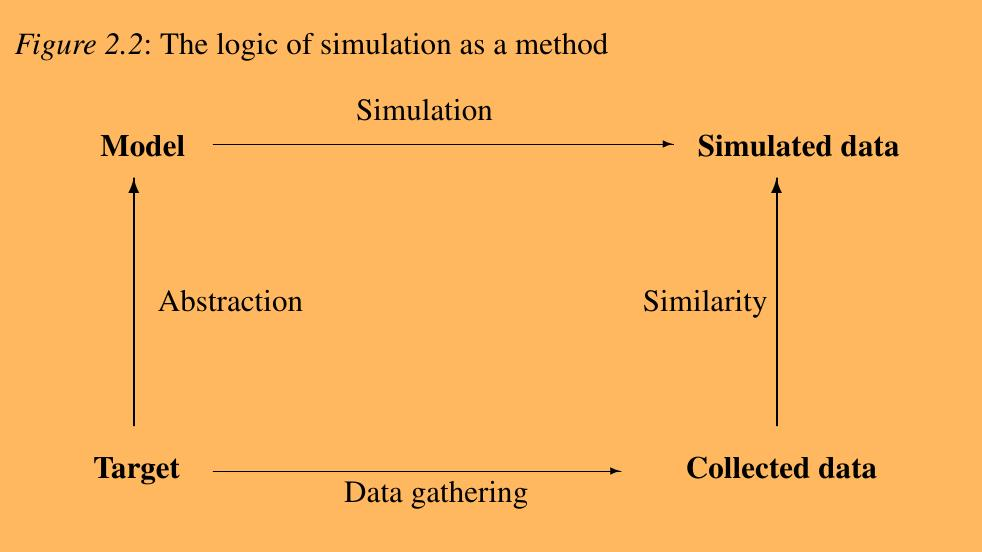
\includegraphics[width=120mm,keepaspectratio=true]{figures/simulationModelling1.jpg}}
\caption{The logic of simulation as a method (after Gilbert 1993)\cite{GilbertTroitzsch}}
%by Gilbert \cite{GilbertTroitzsch}}
\label{fig:SimLog}
\end{figure}

%non covered issues that motivate ABM, 
%TOASK separo més l'explicacio? part1: primers pseudo-agents part2:agents 100%, propietats aconseguides...
\subsection{ABMs in Social Modelling}
With its strong component from software engineering, considering the ABM(Agent Based Modelling) methodology to be applied to social modelling there are some striking features that make it stand out from other paradigms or approaches. ABM copes with the simple and bottom constituents of social science implicated in the modelization of a system, hence it can sometimes allow to describe a system naturally. It is not easy to develop an agent, but you are working with a metaphor  with a structure and concepts that we have at hand everyday. So it is more manageable and natural to express things with that “language” giving more flexibility in the modelization.\\ 
The use of ABM in social modelling allowed to introduce the bottom layer of the hierarchy of concepts of social science, \textbf{people} and all the package of phenomena and issues associated to it. Once you are modelling a person you can work directly with personal or social relationships and their properties, arity, creation and destruction mechanisms, transitivity and interaction rules. This allows to solve models non solved before, like some cooperation, coordination and competition scenarios from game theory where several agents are involved, for instance. Also the direct interaction and feedback effects between the entities and the environment can be represented in the model. Before this step, other paradigms could not cope with the intrinsic phenomena of people interacting in a social scenario. Different issues had to be modelled that were very difficult or impossible to model with raw mathematics.
Social entities, let's say people, or social groups, are not like particles which under the same conditions behave the same way. Two distinguishable entities will act differently under the same conditions. People have different perspectives on their social worlds, have a different knowledge corpus or skills \cite[p.19]{GilbertTroitzsch}. ABMs allows the introduction of this heterogeneity in the models, and also embedding of the Rational Choice Theory \cite{Scott2000}, bounded rationality, and complex cognitive processes. We can give each agent an individualized set of traits, features or methods that will model their different performance in the interactions. We can give them or allow them to catch a different picture from the world, the other agents and themselves.\\ 
ABM is most indicated for describing and simulating a system composed of “behavioral” entities. Whether one is attempting to describe a traffic jam, the stock market, voters, or how an organization works, ABM makes the model seem closer to reality. It is more natural to describe how a party of hunters move in a terrain and circle their preys than to come up with the equations that govern the dynamics of the density of hunters. By the way, because the density equations result from the behavior of hunters, the ABM approach will also enable the user to study aggregate properties\cite[p.2]{Bonabeau2002}; ABM can manage agents at different levels of aggregation. The decission units can be a person but also social entities like families, couples or tribes with their own rules for intearaction and behaviour. You can tune your model easily moving between different layers of abstraction from social sciences. ABM works with models where decission-making and aggregation is clearly separated. The range of complexity of the agent, its behavior, degree of rationality, ability to learn and evolve, and rules of interactions can be tuned more independently of the range of complexity of the aggregation, individualality, and groups. This allows the modeller to work with different levels of description or complexity in the same model\cite[p.2]{Bonabeau2002}.

Also, modelling with agents from a bottom-up point of view will allow to be near the real causes of macroscopic large scale phenomena non predicted from the microscopic local issues. 
% cal afegir això? ``Complex systems theory calls this \textbf{emergence}''. 
Lets mention an example from Helbing,\cite{Helbing2000}; consider a fire escape situation in a confined space: a movie theatre or a concert hall. Let us assume that there is one exit available. How can one increase the outflow of people? Narrowing down the problem, one could ask: what is the effect of putting a column (a pillar) just before exit, slightly asymmetrically (for example, to the left of the exit), about 1 m away from the exit? Intuitively, one might think the column will slow down the outflow of people. However, ABM, backed by real-world experiments, indicates that the column regulates the flow, leading to fewer injured people and a significant increase in the flow, especially if one assumes that injured people cannot move and impede the flow. This result is an example of a \textbf{counterintuitive} consequence of an emergent phenomena: who would think of putting a column in front of an emergency exit? ABM captures that emergent phenomenon in a natural way ( see figure \ref{tab:columnExit} ).\\
\pdfcomment{ATM:el grafic no es una table }
	\begin{table}[ht!]
	\centering
	\begin{tabular}{|c|c|}
		\hline
		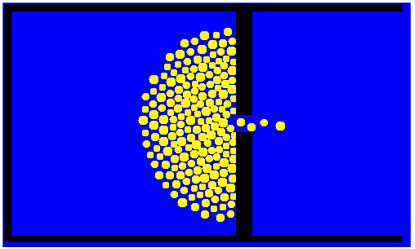
\includegraphics[width=60mm,keepaspectratio=true]{figures/column1.png}
		&
		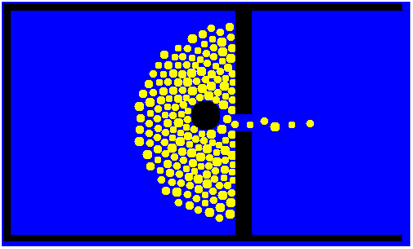
\includegraphics[width=60mm,keepaspectratio=true]{figures/column2.png}\\
		\hline
	\end{tabular}
	\caption{Unexpected emergence of scape patterns under different situations (from \cite{Bonabeau2002}).}
	\label{tab:columnExit}
	\end{table}

\pdfcomment{Cal que parlis de l'avantatge en expressar models a on els agents són heterogenis. D'altra banda, caldria expressar millor que pots introduir processos cognitius avançats fent servir aquesta aproximació, com per exemple mapes mentals del món individualitzats}
\\
\pdfcomment{ATM:done}

Under the next conditions it is advisable, natural and easier to use ABM.

\begin{enumerate}[i-] 
\item The behavior of individuals cannot be clearly defined through aggregate transition rates.
\item Individual behavior is complex. Everything can be done with equations, in principle, but the complexity of differential equations increases exponentially as the complexity of behavior increases. Describing complex individual behavior with equations becomes intractable. For instance, the individual copes with hysteresis\footnote{Hysteresis is the dependence of a system not only on its current environment but also on its past environment. This dependence arises because the system can be in more than one internal state. To predict its future development, either its internal state or its history must be known\cite[p.571–597]{hysteresisDef}.}, or there is heterogeneity in the set of behaviours or there are learning procedures and adaptability.
\item When the interactions between the agents are complex, nonlinear, discontinuous, or discrete (for example, when the behavior of an agent can be altered dramatically, even discontinuously, by other agents).
\item When space is crucial and the agents' positions are not fixed. Example: fire escape, trade, foraging in a stochastic spatial distribution of resources, traffic.
\item Activities are a more natural way of describing the system than processes.
\item Validation and calibration of the model through expert judgment is crucial. ABM is often the most appropriate way of describing what is actually happening in the real world, and the experts can easily “connect” to the model and have a feeling of “ownership”. 
\item Stochasticity applies to the agents' behavior. With ABM, sources of randomness are applied to the right places as opposed to a noise term added more or less arbitrarily to an aggregate equation. 
\end{enumerate}

A last characteristic feature of agent computing, although not often noted, is that once a model has been created it provides not merely one aspect of the solution — the equilibria, say, or the stability — but rather entire solution trajectories \cite{Axtell2000}.\\
\\
\pdfcomment{ATM:next pdfcomment comes from the removed section ABM. ABM section was absorved by section Modelling in Social Sciences}\\
\pdfcomment{Home hi ha molts issues de ABM eh, alguns d'ells discutits al reading group (l'individualisme). Hauries de mostrar aquí algunes de les discussions que hem anat tenint (ben fonamentades i adientment citades, es clar}
\\
\pdfcomment{ATM:molts dels issues grossos surten al PREMO( equif, validacio ), i queden esmentats al paragraf que en parla... Jo anava a afegir issues propis de la metodologia : http://jasss.soc.surrey.ac.uk/12/1/1.html. }

%% TODO
%Issues for ABM applied to social simulation \pdfcomment {ATM : listilla cutre}

%\begin{enumerate}[i-]
%\item Parameter instantiation\\
%      initial population(statistical sampling\? emergence $+$ selection\?)\\
%      initial state of the world at step 0: amount of resources,\ldots \\
%      initial state of the agents? age ditribution,\ldots \\
%\item stop event, time bound,\ldots oscilations \& attractors \ldots
%\item bounded rationality : agents are not megamachines/superman, they commit erros, have mistakes... Not too perfect
%decission making is desirable
%\item validation
%\end{enumerate}


\subsubsection{Epistemology of ABMs in Social Modelling}

Considering specifically archeology, the introduction of modelling led to the first use of these models as emulation of reality. ABM was used to reproduce the patterns in the material samples found. This led to think ABM as a way\pdfcomment{atm: no m'agrada way} of statitistical distribution fitting. ABM models where thought as models that aproximated stochastic variables and patterns in the model. This was the scientific use of ABM. With the idea of producing more accurate explanations of the phenomena, ABM models began to be filled with more details. The objective was to approach the model to reality to obtain nearer outcomes to the data taken as reference. Those first models were designed to be a mirror of reality, and that is why some experts have been calling them Emulation Models. As it is discused by Premo \cite[p.33]{Premo2010} this stalled the usability of models, first due to the difficult of interpreting the causality and processes in a simulation experiment that leads to the arising of phenomena, and second, due to the problem of \textbf{equifinality} \cite[p.31]{Premo2010}.\\
The simulation of a model produces a trace of the states visited by the system. If we execute a stochastic model, the states will be conformed by the exhibited values by the model variables following some distribution. That trace is just only one from all possibles that could appear from the combinations that randomness can produce in the variables. Hence, for a single model and an initial configuration, the stochasticity can lead to many different traces although the system finishes at some atractor state or the same patterns arise. The question is, which trace must be taken into account to explain evidences found in reality? This would be an example of equifinality.\\ 
%
\begin{figure}[h]
\centering
\setlength\fboxsep{0pt}
\setlength\fboxrule{0.5pt}
\fbox{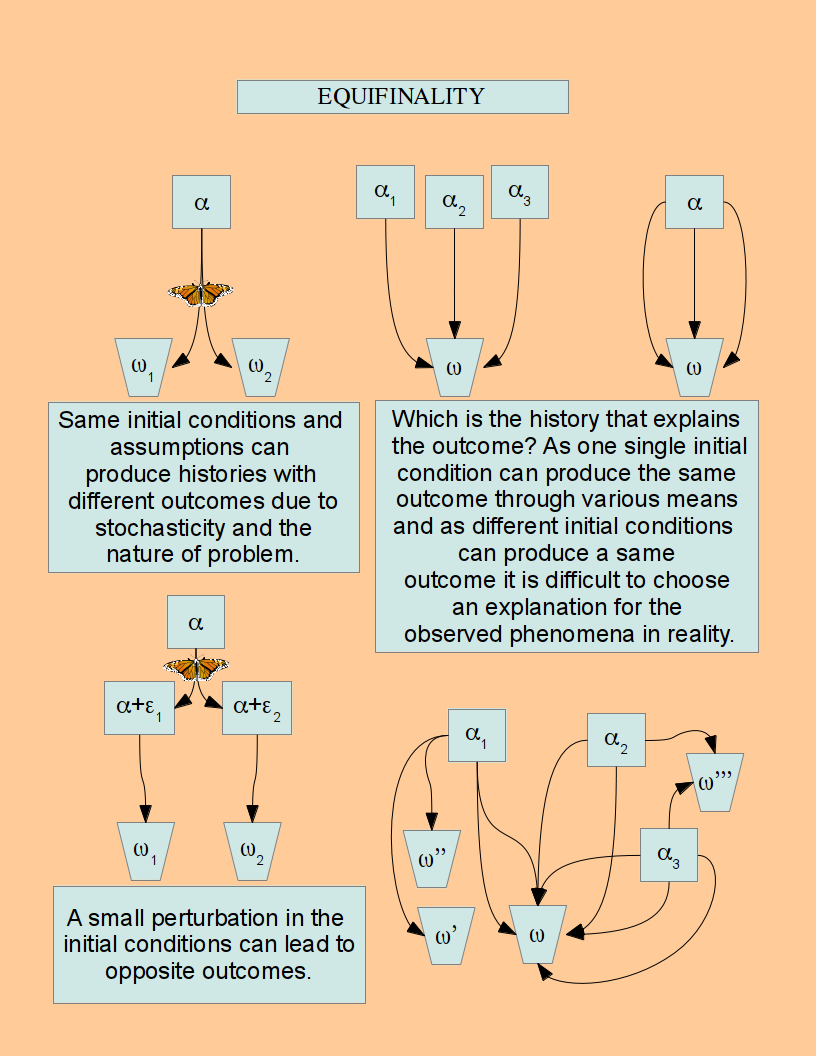
\includegraphics[keepaspectratio=true]{figures/eqf.png}}
\caption{Equifinality in stochastic simulation models. For an initial state 
	with its assumptions $\alpha$ a simulation generates a trace of states 
	that lead to a final state or set of patterns and phenomena $\omega$ (figure based on \cite{Premo2010}).}
\label{fig:Equifinality1}
\end{figure}
%
There is also equifinality when given different initial conditions or assumptions on the model the same outcome is reached. Which is the initial escenario that produced the evidences? Due to the long time of the history trace, all initial conditions could have the same probability and data does not makes easier the discrimination. Equifinality also appears when the system exhibits sensitivity to initial conditions. Sensitivity is a typical trait of \textbf{complex systems} and it is commonly known as the \textbf{butterfly effect}. A small perturbation, that is considered \textbf{negligible}, in a initial condition can produce a trace with opposite conclusions respect another 
one without that perturbation. Furthermore, due to sensitivity again, an initial condition in different runs belonging to a same simulation experiment will have usual small perturbations appearing as differences between different traces. Sensitivity to these small inner perturbations can lead to opposite outcomes in the experiment making it difficult to extract and deduce the common patterns or general behaviour we desire to check against data. It will be harder to separate noise from information. The same listed issues hold when instead considering several initial states or assumptions we consider diverse models as candidates for the explanation.\\
%
% different models can explain the outcome, which model must be chosen? -> EQF
%
% . y aixo es un unsustainable situaion per a extraccio espitemologica. No pots deduir una llei general, perque es inestable...
%
%And that is an example of equifinality. ... mention the other cases ... need to reduce detail .... another
%epistemological target and strategy -> Explor. Models ... explo mod features
% 
%
There is another alternative to replicating evidence, another way of exploiting ABMs within another epistemological strategy descrived by Premo \cite[p.33-34]{Premo2010} named \textbf{Exploratory Models}. Models can be simplified to the bone. This would keep the most essential processes related to the scientific question that motivated the simulation. As it is said above\ref{myPremo_simplicity}, a simple model allows a clearer insight of what is happening, and of the path of causality between the constituents and the phenomena. Then, taking advantage of equifinality, the use of the model is to explore causality and tendency in the different traces, how happens the connection between assumptions and parameters with phenomena and states. Simplicity in the model allows to design controlled experiments and very explicit and bounded assumptions for hypothesis generation about the model to enhance the knowledge of the processes we model from reality. Then, these experiments will explore the space of parameters under sensivity to detect ranges, tendencies or configurations that produce patterns similar or far from the empirical observations.\\ 
% data contrast : initial assumptions revision -> hypoth revision -> new experiments -> loop -> refine theory & hypothesis 
%generation of hypoth linked to abduction/retroduction, Premo pg 34, last paragraph
The connection between hypothesis, assumptions and outcomes is studied by the modelers applying \textbf{retroductive reasoning}\cite[p.34]{Premo2010}. Retroductive reasoning, also known as \textbf{abduction} is an inference frame that connects effects with its causes in a coherent way with an a-priori theory. The best example to catch the concept is to show it compared to other syllogisms.\\ \textbf{Deduction} makes explicit the facts that some premises entail through some general rules. Given that \textit{``all human are mortal''} and \textit{``Socrates is a human''} I state that \textit{``Socrates is mortal''}. You could see this as a kind of prediction engine. \textbf{Induction} produces the general rules, it is an abstraction inference process. For some set of sampled particular cases $x_i$ I observe both properties, \textit{``$x_i$ is mortal''} and \textit{``$x_i$ is a human''}. Then, I could express this correlation inducing the rule \textit{``all mortals are human''} or \textit{``if someone is mortal then it is a human''}, but as we all have seen flies and ants dying, the statement would cover incorrect cases. The final produced general rule shall be \textit{``all human are mortal''}. Abduction tries to discover the facts that act as cause for some observed evidences. This inference process produces a causal \textbf{explanation}. For instance, I find a dead entity $e$, \textit{``$e$ is mortal''}. I have at hand my a-priori knowledge about the domain, \textit{``all human are mortal''}, and produce my explanation : \textit{``$e$ is mortal''} because \textit{``$e$ is a human''}. That is a plausible explanation, but as shown above, flies and ants are also mortal and it is plausible to say \textit{``$e$ is mortal''} because \textit{``$e$ is an ant''}. Explanation must be refined. Observations and hypothesis trigger new hypothesis to be included in the retroductive inference. New evidences produced by experiments will filter explanations that will allow decide wheter $e$ is a human or an ant. According to Peirce, retroduction can provide good reasons to pursue a hypothesis but does not, by itself, provide good reasons to believe the hypothesis. In successful applications of retroduction, pursuit leads to the accumulation of evidence that will fix the remaining accepted hypothesis for the explanation \cite{Peirce_Abduction}.\\  
%
%Surprising phenomenon P is observed
%If hypothesis H were true, H would explain why P would be expected
%Therefore, there is reason to suspect H may be true.
%Things go this way? --->
%Many experiments, observe many times H and P appearing : There is a causal connection H |- P, tested
%through deduction; induce the explanation H->P. Retroduction working with the help of induct+deduct
%
% experiments -> induce rules from param explor -> check them with retroduction
%
%the set of assumptions and hypothesis states a set of a priori rules 
%the causality connection of the constituents will also induce a set of these normic rules(e.g. all birds fly)
%the explanation process is retroduction aplication searching for the plausible chain of rules
%that produced the facts and patterns of the outcome
%
The explanation of the outcome and the evidences from reality arises from the assemble of the knowledge and evidences we gather from experiments. The model becomes part of a pragmatic reductionism frame, what we comprehend from the inner processes is integrated for the comprehension of the whole. This comprehension will induce new questions and hypothesis (or purge them) that will motivate new experiments and modelling tasks producing a loop of model refinement. Generation of these new hypothesis and questions will also be of profit for theory improvement or theory building and self-criticism in a loop of modelization and question-discovering feeding each other. \pdfcomment{ATM:cada 3 frases hauria de posar una ref a Premo, es excessiu? faig referencia en un punt i dic q tot el que he posat ve d'alla?}.\\ 

%When you construct a model you must think how will you use it, how will you apply it to a rational process 
%for knowledge production. 
%You must give another epistemological use to your models. Another strategy to these techniques.... Explo Models
%do not replicate evidence, but investigate processes and interaction
%ontological reductionism : MODEL({p1,p2,...p_n}) vs system
%pragmatical reductionism : MODEL(p1)+MODEL(p2)+...+MODEL(p_n) vs system

\begin{figure}[htb]
\centering
\setlength\fboxsep{0pt}
\setlength\fboxrule{0.5pt}
\fbox{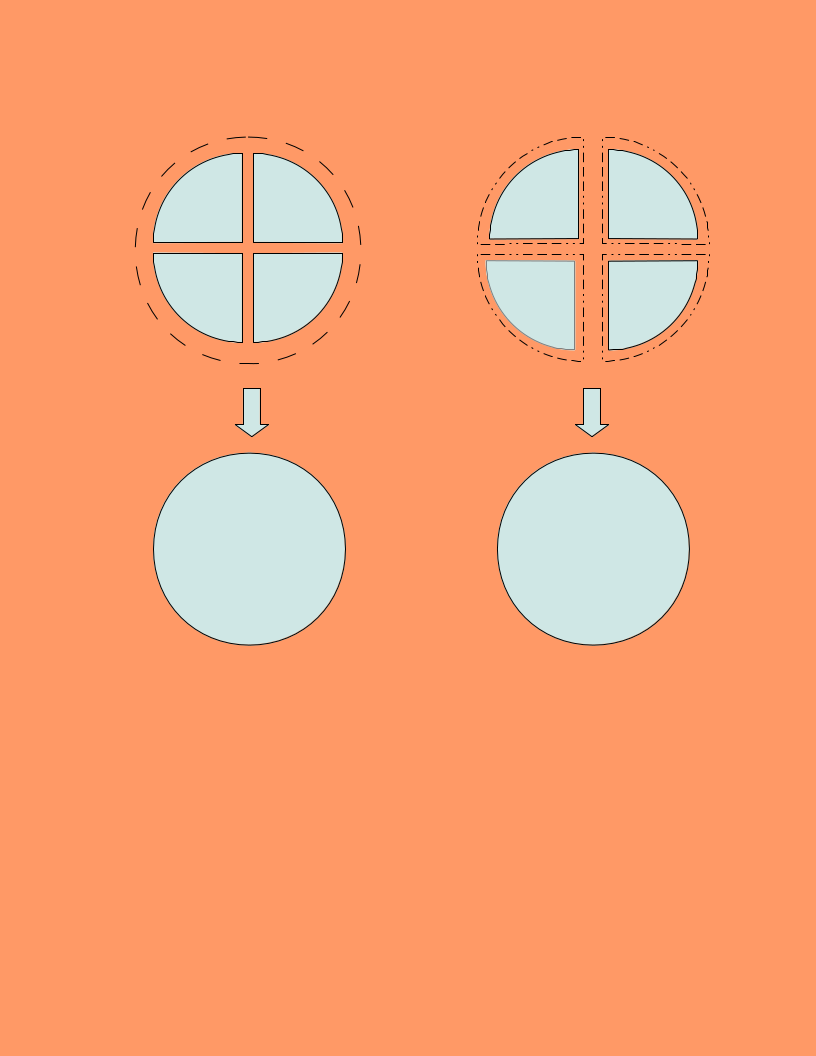
\includegraphics[width=120mm,keepaspectratio=true]{figures/pragmaticReduct.png}}
\caption{Ontological Reductionism vs Pragmatical Reductionism.}
\label{fig:Equifinality2}
\end{figure}

%
%Modelling methodology will be materialized through the framework of simulation technique. It will follow a series
%of stages defined in simulation-based research. 

%\begin{description}
%\renewcommand{\labelitemi}{$\bullet$}
%\renewcommand{\labelitemii}{$\cdot$}
%\item [Definition of the target] A purpose for the model or a question over the target system is stated.
%	\begin{description}
%	\item [prediction/prognosis]
%	\item [diagnosis]
%	\item [theory validation / discovering]
%	\item [study future possible worlds]
%	\end{description}
%\item [Observations] Data gathering, parameters and initial conditions retrieval from the target system using %bibliography, interviews and experts' supervision.
%\item [Assumptions] Relevant simplifications are considered. 
%\item [Design model] Translation of the experts' conceptualizations to a formal modelling language or structure. 
%\item [Computer programming] Implementation of the model.
%	\begin{description}
%	\item [verification] Test that the program matches the specifications and features of the formal model.
%	\end{description}
%\item [Run simulation] Perform the experiments.
%\item [Gather results] Extract conclussions from the simulation data. 
%\item [Validation] Check that the conclussions are scientifically sound and match the plausible target system behaviour. The model should behave similar to the target system under the selected features and details.
%	\begin{description}
%	\item [sensivity analisys] Detect variables and parameters that produce great oscilations on the simulation results.
%	\end{description}
%\end{description}

%%********************************************************

\subsection{Summary checklist}

The next checklist sumarizes the steps visited along the process of development and execution of our model. The ABM methodology fits in the the series of defined stages for simulation based research. 

\begin{description}
\renewcommand{\labelitemi}{$\bullet$}
\renewcommand{\labelitemii}{$\cdot$}
\item [Definition of the target] A purpose for the model or a question over the target system is stated. The model will be aimed to prediction or prognosis; diagnosis, to construct an explanation for the dynamics or the state of the system; it also can be aimed to theory validation or theory discovering, or study future possible worlds configurations or atractors in the system.
\item [Observations] Data gathering, parameters and initial conditions retrieval is done from the target real system using bibliography, interviews and experts' supervision.
\item [Assumptions] Relevant simplifications or principal concepts are considered. 
\item [Design model] Translation of the experts' conceptualizations to a formal modelling language or structure. 
\item [Computer programming] Implementation of the model in a computational language. A verification phase will test that the program matches the specifications and features of the formal model.
\item [Run simulation] Perform the experiments. The runs will generate the traces that will conform the picture of the exploration space for the stochastic variables in the system and the emergent top level phenomena.
\item [Gather results] Extract conclussions from the simulation data, stablish correlations and dynamics. This phase will allow to detect evidences for new hypothesis and conclussions or their discarding.  
\item [Validation] Check that the conclussions are scientifically sound and match the plausible target system behaviour. \textbf{Sensivity analisys} will help detect variables and parameters that produce great oscilations on the simulation results and extract issues for the loop of model, theory and hypothesis refinement.
\end{description}
%%********************************************************


%%TODO GRAFIC del "cicle``

\begin{figure}[h]
\centering
\setlength\fboxsep{0pt}
\setlength\fboxrule{0.5pt}
\fbox{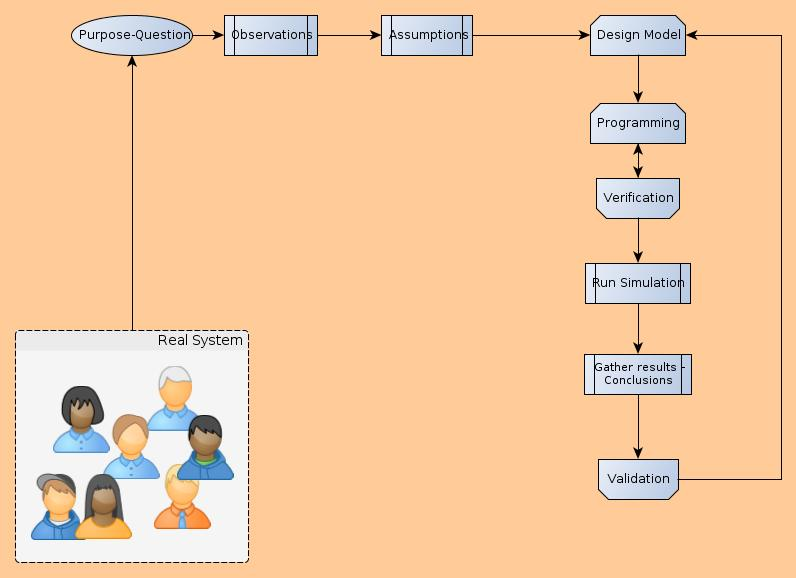
\includegraphics[width=120mm,keepaspectratio=true]{figures/simulationMethodlogy.jpg}}
\caption{Stages defined in simulation-based research \cite{RussellNorvig}}
%by Gilbert \cite{GilbertTroitzsch}}
\label{fig:SimStages}
\end{figure}


%bridge to ABM section

%%%% end content


% TOASK afegir certs apartats de l'ODD??? adaptar les descripcions dels apartats de l'ODD\\


%%%%%%%%%%%%%%%%%%%%%%%%%%
\section{Conceptual Framework}

This section introduces some definitions and explanations about the main needed concepts to expose the design of the model for the issues and questions stated in chapter one. The text begins explaining what agents consist on. The description of agents from AI covers their architecture and competences, and how different techniques and paradigms endow them with the diverse features and capabilities to solve the problems they are programmed for. An explanation about complex systems follows the section of multi agent systems. It is a necessity due to the nature of the problem and the properties exhibited by models consisting in multiple agents interacting each other. The section links typical complex system phenomena to the arising properties of the models studied for the topics of these master thesis. Emergence is defined and stressed in a dedicated subsection. This part finishes giving some brief ideas about what evolution is. The topic is introduced due to the evolutive component in the model to be run in the simulations. We seek to observe how either of the strategies adapts to the changing environment and how the dynamics favors one instead of the other producing adaptative changes in the agents. As we will study the different social groups in a competitive environment the section will introduce the concept of coevolution, the mutual feedback of evolutive changes between neighbour adaptative groups of entities.After this definitions the next part will retake the topic of agents in the section about Agent Base Models to introduce more ideas and issues from Multi Agent Systems and social simulation.   


\subsection{Multi Agent Systems} %% M.A.S.

%% aqui poses tota la part mes tecnica/teorica dels agents, a ABM ja no caldra explicar-ho
%% ABM explicara issues de modelatge i aplicacio cientifica

%% Agent System : equal agents in a shared environment
%% Multi Agent System : Heterogeneous agents.
%% TODO refina definicio 

%% definition
Multi Agent System(MAS) is an architecture for software development based on designing a solution for a problem that 
executes of a set of computational entities called agents that interact themselves in a defined environment\cite[chapter.1]{Wooldridge2002}.\\
Such entities are active decission making actors in the modelled system. The modelling lifecycle of an MAS will consider a stage where decission making processes must be identified from the system. Usually those decission making actions are carried along by more or less clear individual entities from the system. The modelling process will take the task to set the matching between these entities and the agent that will form the MAS. The concept ''agent`` condenses a set of features that will specify the modelling metaphor that an agent represents:
some enclosed set of mechanisms to be aware of the state of the system, a set of goals to accomplish and the engine to decide from a bounded perception of the world, the actions to apply on it to achieve these goals. Besides the reasoning component of the agents, MASs have a strong component of inter-agent relationship. How one agent interacts with other agents could as important or more as how it reacts to world changes.

%%bottom-up approach, reductionist way of looking at the things, we try to understand the parts\\
%%to join them from their relationship and then we try to get the big picture.

\subsubsection{Agents}

%%TODO TOASK definir nomes el necessari per a la comprensio dels ABMs? anar mes enlla i tocar features q no
%% ens son rellevants??

%%---------agents, una component que dispara la no linearitat i per tant la complexitat\\
%%---------heterogeneitat : dos \`atoms de Carboni es comporten igual en mateixes condicions, les persones no.\\

%%refine

An agent is a computer system that is capable of independent action on behalf of its user or owner,
figuring out what needs to be done to satisfy design objectives, rather than constantly being told.\cite[ch.1]{Wooldridge2002} An agent solves problems applying iteratively the schema of sense, decide and 
act continously. Each of the steps can add new targets to fulfill which will keep the agent exploring 
the environment and interacting with it and other agents to develop its strategies to solve the tasks 
and achieve goals.\\

Agents are \cite[p.115-152]{WooldridgeJennings1995}:
\begin{enumerate}[i-]
 \item clearly identifiable problem solving entities with well-defined boundaries and
interfaces;
\item situated (embedded) in a particular environment—they receive inputs related to the
state of their environment through sensors and they act on the environment through
effectors;
\item designed to fulfill a specific purpose—they have particular objectives (goals) to
achieve;
\item autonomous—they have control both over their internal state and over their own
behaviour;
\item capable of exhibiting flexible problem solving behaviour in pursuit of their design
objectives—they need to be both reactive (able to respond in a timely fashion to
changes that occur in their environment) and reactive (able to act in anticipation of
future goals).
\end{enumerate}


	\begin{figure}[h]
	\centering
	\setlength\fboxsep{0pt}
	\setlength\fboxrule{0.5pt}
	\fbox{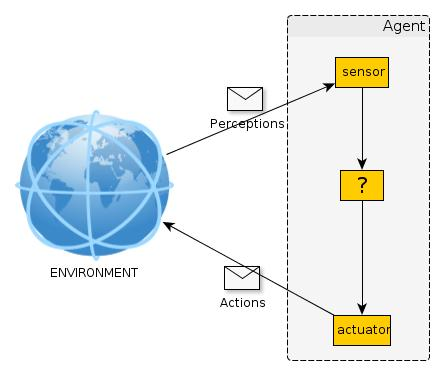
\includegraphics[width=60mm,keepaspectratio=true]{figures/agentArchitect0.jpg}}
	\caption{Agents interact with environment through sensors and actuators.}
	%by Wooldridge2002 \cite{Wooldridge2002}}
	\label{fig:AgWool}
	\end{figure}

%% what is nicer? picture or algorithm?
%% 	\begin{algorithm}[H]
%%	\SetAlgoSkip{} 
%%	\SetAlgoLined
%%	initialization\;
%%	\While{not end}
%%	{
%%		s = read environment current state\;
%%		a = getAction(s)\;
%%		launch(a)\;
%%	}
%%	\caption{Agents basic main loop.}
%%	\end{algorithm}

An example of a very simple agent would be a thermostat. It samples the environment with a probe/sensor, 
checks if the temperature corresponds to the desired one. According to the measure it launches one of the two 
actions, to set the heater to ON or to OFF.\\
But we could have something as complex as an agent representing a car in a traffic simulation while drives 
from one point to another in the city. The agent would have accesible a knowledge base of traffic rules 
constraining its actions. The agent at each time step of the simulation would control the swarm of other 
vehicles to avoid collisions and would follow paths and perform actions coherent to the rules of traffic. 
The traffic rules would act as middle interface consensus of fair driving that coordinates all the cars 
and allows some prediction of the adjacent cars. The agent can be designed a step further. When congestion 
increases to a predefined threshold, which could be tuned through authomatic learning, the agent recalculates 
the route to adapt and avoid the traffic jam.\\
Intelligent agent design considers the setting of Perceptions, Actions, Goals and Environment. These
aspects form a general structure where an agent design can grow. Mentioning an example considering a 
system that simulates hunting practices from ancient cultures will show how features from the agent are 
attached to these modules in the structure(table \ref{tab:hunterAgentSetting}).\\
	\begin{table}[h]
	\centering
	\begin{tabular}{|l||l|}
		\hline
		\textbf{Perceptions} & Hunger, TerrainSlope, ReadTracks, LookForPrey.\\
		\textbf{Actions} & Eat, LightFire, Cook, ThrowArrow, Walk, Run, Stalk, Hide.\\
		\textbf{Goals} & Survive, AvoidHarm.\\
		\textbf{Environment} & Weather, Plants, Mountain, Valley, Caves, Deers, Rabbits.\\ 
		\hline
	\end{tabular}
	\caption{Setting table for a hunter agent.}
	\label{tab:hunterAgentSetting}
	\end{table}

%%TODO TOASK cal ser tant pedagogics i esmentar quins designs hi ha?
%% endow with task-solving -> reasoning -> Agent Design
%% endow with interaction managing -> society design -> MultiAgent Systems Design

%%\subsubsection{Agent Architecture Specification}

\paragraph{Agent brief formal description}
	
Let E be an environment with a finite set of states 
\begin{equation}
	\Omega = \{\omega_0,\omega_1,\ldots \}
\end{equation}
Each agent has available a set of actions 
\begin{equation}
	A = \{ \alpha_0, \alpha_1, \ldots \} 
\end{equation}
An action is a function that changes the state of the environment 
\begin{equation}
	\alpha_i : \Omega \longrightarrow \Omega 
\end{equation}
An agent's run is a sequence of states of the environment where the transitions were triggered 
by actions launched by the agent. Let $R$ be the set of all possible runs over $\Omega$ and $A$, and
$r^{u}$ one sequence of length $u$.
\begin{equation}
	r^{u} = ( \omega_0 , \alpha_0 , \omega_1 , \alpha_1 ,\ldots, \omega_{u-1} , \alpha_{u-1} , \omega_u )
\end{equation}
Let $R^{A}$ the sequences that end with an action 
\begin{equation}
	r^{u-1}_{A} = ( \omega_0 , \alpha_0 , \omega_1 , \alpha_1 ,\ldots, \omega_{u-1} , \alpha_{u-1} )
\end{equation}
Let $R^{\Omega}$ the sequences that end with an environment state 
\begin{equation}
	r^{u}_{\Omega} = ( \omega_0 , \alpha_0 , \omega_1 , \alpha_1 ,\ldots, \omega_{u-1} , \alpha_{u-1} , \omega_u )
\end{equation}
Actions in the run are the response of an agent $X_i$ to the states of the environment
\begin{equation}
	\forall j \in [0..u-1] : X_i(r^{j}_{\Omega}) = \alpha_j
\end{equation}
An stochastic and historic dependent environment behaviour, $\tau$, can be described as
\begin{equation}
	\tau : R^{A} \longrightarrow \wp(\Omega)
\end{equation}
A Markovian environment behaviour would be defined as
\begin{equation}
	\tau : \Omega,A \longrightarrow \wp(\Omega)
\end{equation}
and the next would hold for the runs
\begin{equation} 
	\forall i \in [0..u-1] : \tau(\omega_i, \alpha_i) = \omega_{i+1}
\end{equation}
Let's say that no end condition is described for the runs here because althought it could happen
$\tau(\omega_i, \alpha_i) = \varnothing$, many other conditions could mark the end of a run.
For instance, a run can finish because the population of agents reaches 0 due to some dying process.
A run can also stop after a finite number of transitions, or some predefined event appears.\\
\\
An agent $X_i$ retrieves information from the history of environment states to choose an action to launch
\begin{equation}
	X_i : R^{\Omega} \longrightarrow A 
\end{equation}

%%

\paragraph{Agent Main Behaviours}

There is a set of key points that an agent should accomplish to go beyond a simple AI application, a problem solver, or just a system process. AI has compiled some asked mandatory behaviours lisked below to a software to be considered an agent \cite[ch.2]{Wooldridge2002}\cite[ch.1, ch.2]{RussellNorvig}. 

\begin{description}
	\item [Autonomy] Other entities do not set the agent objectives nor decissions. With agents, 
	we give a high-level description of the delegated goal, and let the control mechanism figure
	out what to do, knowing that it will act in accordance with some built-in theory of rational 
	agency to satisfy it.

	\item [Reactivity] Response to environment stimulus or changes. A reactive agent is 
	one that maintains an ongoing interaction with its environment, and responds to changes 
	that occur in it (in time for the response to be useful). A pure reactive agent, the 
	thermostat can be formally descrived as
	\begin{equation}
		X_i : \Omega \longrightarrow A 
	\end{equation}
	\item [Proactivity] It means anticipation, taking initiative, detect oportunities. This
	could materialize in prediction of a future event an realize a set of a priori actions 
	before it occurs. For instance, if you are modelling a population of farmers and agent A1 
	sees the state of low resources of its neighbour agent A2 at the end of the season. As 
	a social action, A1 makes a pressent of food to A2 before it begins to starve or asks for
	help. We also know that this kind of action will produce stronger bonds and could have their
	pay-off in the future. But the most extended example is when you enter in a bookshop, 
	as you delay a bit in your search, a salesman appears offering its help before you ask for it.
	It could mean that the agent produces a set of actions that trigger an environment event
	that will allow the execution of an action the approaches the agent to its goals.

	\item [Social capabilities] Cooperation, coordination, negotiation, competition, and mind models.
	Some objectives are not achievable by the only means of the agent. The agent must interact
	with other entities that can produce the chain of actions to produce the changes in the
	environment needed.
	%conflict
	Agents inhabit and intearact with the environment applying actions and producing effects
	in a same medium. Goals, effects and dynamics can clash. Is it possible the appearance of
	conflict. Goals and planned trend can be contradictory for more than one agent. According
	to the model of negotiation of the agent it can try to change its plan trying to not interfere
	with the other agents, or produce a deliberate interference or ignore it and stick to its
	objectives.
	Social capabilities will cover the spectrum of comunication but also integrate the other agents
	behaviour. Some sophisticated agents include mind models to add, predict the other agents' 
	behaviour in its knowledge representation engines.
	\begin{description}
		\item [Cooperation] Cooperation is working together as a team to achieve a shared goal.
		Often prompted either by the fact that no one agent can achieve the goal alone, or that 
		cooperation will obtain a better result (e.g., get result faster). That is very easy
		exemplified with hunt parties or some families of farmers that while one member takes care
		of the plot the other takes the cattle for grazing.

		\item [Coordination] Coordination is managing the interdependencies between activities.
		For example, if there is a non-sharable resource that you want to use and I want to use, 
		then we need to coordinate.

		\item [Negotiation] Negotiation is the ability to reach agreements on matters of common 
		interest. At the appearance of conflict a solution that benefits the parts is searched.
		For example: Two farmers arrive at a piece of land good for crop growing. A possible deal: split
		the land in two.Another solution : both work on the land, but each has assigned different
		tasks. By the end of the year they divide the harvest. Typically involves offer and 
		counter-offer, with compromises made by participants.

	\end{description}

	\item [Learning] Prediction for future situations,reuse solutions,avoid past errors. The agents stores
	patterns from the history of environment changes, or other agents' actions. The patterns induce a model
	of the world or of the task to perform used by the agent for future actions. As a detail, although the 
	learning could be produced in first stages of the run to produce benefits along the life of the agent,
	it is desirable that the learning should occur along all the run to produce a real adaptation of the 
	agent. The keyword is \textbf{incremental learning}.
\end{description}

%% extra properies:Mobility,Veracity,Benevolence,Rationality,Learning/adaption.

\paragraph{Intelligent Agents Architecture}

This paragraph will show different decompositions of how an agent is structured 
and provide an answer to the question of how the sensor data and the current internal 
state of the agent determine the actions and future internal state of the agent.
The thermostat example contains an environment with a bounded and tractable number of states.
Such situations can be solved with a direct implementation setting the bijective function 
state - action with a table or with a limited number of rules.
As complexity of modelled systems grows, the number of states and possibilities become
untractable. Theres no time nor space to specify each correspondence. The agents apply different 
techniques for retrieving features and structure from the environment to proceed with the
decission process from an abstraction to the action to perform \cite[ch.2]{RussellNorvig}.  

\begin{description} %% we are interested in this division
	\item Reactive Architectures

The decission process in Reactive Architectures selects actions only based on the last perception retrieved
from the environment. It does not considers any subset of past perceptions. Reactive Architectures encompass  
the Simple Reflex Agents.

		\begin{figure}[h]
		\centering
		\setlength\fboxsep{0pt}
		\setlength\fboxrule{0.5pt}
		\fbox{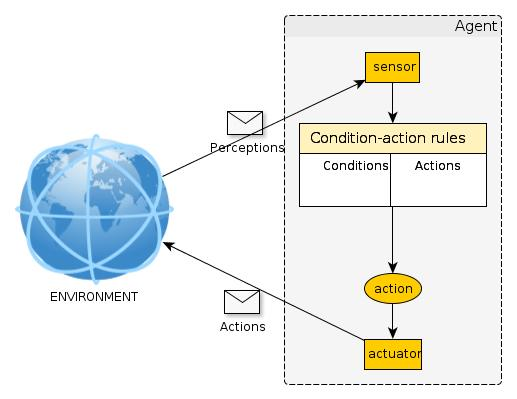
\includegraphics[width=80mm,keepaspectratio=true]{figures/SimpleReflexArchitect0.jpg}}
		\caption{Simple Reflex Agent Architecture}
		%by RussellNorvig \cite{RussellNorvig}}
		\label{fig:SimpleReflexArchitect0_label}
		\end{figure}

A change in the environment provokes a response from the agent. When changes and deliberations in agent are
only motivated by an event in the environment, the agent is pure reactive.\\
	
		\begin{algorithm}[h]
		\SetAlgoLined
		\SetKwData{rules}{rules}\SetKwData{rule}{rule}\SetKwData{I}{I}
		\SetKwFunction{getNextPercept}{getNextPercept}\SetKwFunction{brf}{brf}\SetKwFunction{options}{options}\SetKwFunction{filter}{filter}\SetKwFunction{plan}{plan}\SetKwFunction{execute}{execute}
		\BlankLine
		\While {true}{
			$\sigma$ $\gets$ getNextPercept()\;
			$rule$ $\gets$ ruleMatch($rules$, $\sigma$)\;
			$\alpha$ $\gets$ ruleAction($rule$)\;
			execute($\alpha$)\;
		}
		\caption{Simple Reflex Agent main loop}
		\end{algorithm}

	\begin{itemize}
		%%refine \item With Internal state vs without internal state

		\item Cognitive Maps
		\item State Transition Machines %% TODO mira exemple

		\begin{figure}[h]
		\centering
		\setlength\fboxsep{0pt}
		\setlength\fboxrule{0.5pt}
		\fbox{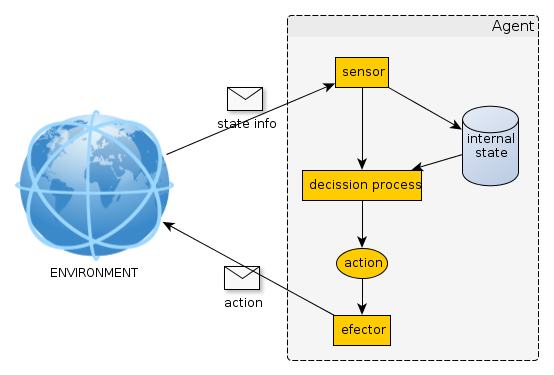
\includegraphics[width=80mm,keepaspectratio=true]{figures/agentArchitect1.png}}
		\caption{State Machine Reactive Agent Architecture}
		%by Wooldridge2002 \cite{Wooldridge2002}}
		\label{fig:StateMachine}
		\end{figure}

		\item if-then rules
	\end{itemize}
	
	\item Deliberative Architectures

	A deliberative agent uses symbolic reasoning to deduce the action to launch. The deliberative agent
	contains explicitly the goal that steers its behaviour. Deliberation is done through an internal formal 
	representation of the state of the world, the state of the agent and other information retrieved by
	it. A logic engine will produce deductions from the facts stored in the agent memory, the knowledge
	base. The perceptions from the environment become facts to add to the internal representation of
	the environment. From this internal world model the agent can deduce trends for prediction besides
	the next action to launch. A state of the environment or of the agent is specified. The agent must find 
	the way to fulfill this within his reach of perceptions and actions. Desirable situations are seeked, 
	called goals, that is environment states or agent states. 

	Given some systems or situations, goals are non achievable from a single action execution. The agent 
	must apply search and planning techniques to conform a plan that will satisfy, after a limited number of 
	steps, the desired goal.

	Goals could be a design feature of the agent, for instance \textbf{survive} \& \textbf{reproduce}, or could 
	be set dynamically in runtime by conditions in the environment or through user commandment.

	\begin{description} 
		\item [Logic] Deliberative agents will use assert clauses and structures to represent facts in 
		a logic of some level, CP0, CP1. Each new change in the knowledge base will allow to deduce
		new facts from the status of the system to check againts the goals and other issues the agent
		is considering to produce an action coherent with the planning and the mechanics of the environment
		to fulfill a new step to get nearer to the goals.
		%%TODO dibuix de la taula i els objectes mes la representacio interna : on(), above(),under()
		The agent will use its knowledge base as a theory of the world and things plus the dynamic facts
		that represent the volatile states.\\
		Let $\rho$ be a theory of the world. Depending on the architecture this can be a set of rules,
		or a learned structure along the run.\\ 
		If $\Gamma$ is a description for the current state of the world. $A$ the set of possible actions 
		\{$\alpha_1$, $\alpha_2$, $\alpha_3$, \ldots\}. And $\Gamma \vdash_{\rho} \Phi$ stands for a succesful 
		prove that $\Phi$ is deduced from the knowledge base $\Gamma$ using theory $\rho$. The Deliberative 
		agent will choose actions according to a schema like that:

		\begin{algorithm}[H]
		\ForAll{$\alpha \in A$}{	
			\If{$\Gamma \vdash_{\rho} doAction(\alpha)$}{
				\Return $\alpha$;
			}
		}

		\ForAll{$\alpha \in A$}{	
			\If{$\Gamma \nvdash_{\rho} \neg doAction(\alpha)$}{
				\Return $\alpha$;
			}
		}
		\Return null;
		\end{algorithm}

		Asserts from Logic will be used to state the facts that are true from environment
		and the other agents.
		% Knowledge representation. Solvers : Resolution, Forward/Backward chaining
		
		\item [BDI] BDI stands for Belief-Desire-Intention. Yoav Shoham introduced “agent-oriented 
		programming” in 1990 \cite{Shoham1990}:“new programming paradigm, based on a societal view of
		computation”. The key idea is about directly programming agents in terms of \textbf{intentional}
		notions like belief, commitment, and intention.	Beliefs are used to model the state of the world.
		Desire allows the selection of possible states of the world and preferences. Intentions are 
		compromises to achieve a given state, they are the commitment of the agent.

		BDI belongs to a overloaded kind of logics called modal logics which add meta language operators to
		the facts to alter with some nuance the meaning or the semantic interpretation of the fact.
		For instance, let $\phi$ be a fact that could represent ``deer is in the wood''. Indeed it is true
		for the example. Our agent has not seen it and only has some clue that the deer is in the 
		wood; so the agent states $\Box_B \phi$, with an operator $\Box_B$ to indicate ``I believe the 
		deer is in the wood''. The memory of the agent will contain also the facts below
		  \begin{description}
		    \item[$\theta$] = ``I am hungry''.
		    \item[$\eta$] = ``I go hunting''.
		    \item [$\Box_D \eta$] = ``I have Desire for going hunting''.
		    \item [$\Box_I \eta$] = ``I have Intention for going hunting''.
		  \end{description}
		Some of these entail from other. They are governed by the next rules from the knowledge base
		\begin{itemize}
		\item myState(HUNGRY) 
			$\rightarrow$ $\Box_D$ doAction(HUNT)
		\item $\Box_D$ doAction(HUNT) $\wedge$ $\Box_B$ entityAtPlace($x$,$y$) $\wedge$ edible($x$)\\ 
			$\rightarrow$ $\Box_I$ doAction(HUNT)
		\item $\Box_I$ doAction(HUNT) $\wedge$ $\Box_B$ entityAtPlace($x$,$y$) $\wedge$ edible($x$)\\ 
			$\rightarrow$ doAction(go, $y$)
		\item entityAtPlace(MYSELF,$p$) $\wedge$ $\Box_I$ doAction(HUNT) $\wedge$ entityAtPlace($x$,$y$) $\wedge$ edible($x$) $\wedge$ distance($p$,$y$) $\leq$ HUNTDISTANCE	
			$\rightarrow$ doAction(HUNT,$x$)
		\item doAction($a$,$x$) $\rightarrow$ launchAction($a$($x$))
		\end{itemize}

		This rules would carry the agent to satisfy the goal of feeding going through the goal of going where the
		prey is, and see that it is indeed there where the agent believed.

		Programming agents this way allows a deeper description of the dynamics around the goals an agent 
		self-imposes and also an easier way for the agent to reason about the other agents. This last point
		is crucial for a better integration of the social dynamics in the planning of goal achieving. The agent
		can construct through facts of Believing, Desire and Intention a mind model of the other models taking
		into account their BDI intentions and adapting to them to cooperate or compete. 

		Continuing the example, the agent would be inmersed in social deliberations after retrieving from the
		world facts like $\Box_{I}^i \eta$ that stand for ``Agent $i$ has the Intention of hunting''. The 
		interaction of all these facts, entityAtPlace(MYSELF,P), entityAtPlace($i$, P) will make deduce to the
		MYSELF agent somekind of communication protocol with agent $i$ to solve the conflict. Because they could 
		end to hunting the same deer, before they would launch their HUNT action, they must reach a consensus about
		what to do each other. 

		Schema for BDI	

		\begin{algorithm}[H]
		\SetAlgoLined
		\SetKwData{B}{B}\SetKwData{D}{D}\SetKwData{I}{I}
		\SetKwFunction{getNextPercept}{getNextPercept}\SetKwFunction{brf}{brf}\SetKwFunction{options}{options}\SetKwFunction{filter}{filter}\SetKwFunction{plan}{plan}\SetKwFunction{execute}{execute}
		\BlankLine
		$B \gets B_0$\;
		$I \gets I_0$\;
		\While {true}{
			$\delta$ $\gets$ getNextPercept()\;
			$B$ $\gets$ brf($B$, $\delta$)\;
			$D$ $\gets$ options($B$, $I$)\;
			$I$ $\gets$ filter($B$, $D$, $I$)\;
			$\pi$ $\gets$ plan($B$, $I$)\;
			execute($\pi$)\;
		}
		\caption{BDI main loop}
		\end{algorithm}

		%other issues about BDI : planning of actions to fulfill intentions, and commitment management

		%TODO add the second algorithm?

		\item[Utility based]

		Goal-based models are a dycothomic approach that rely on bivalued logics. A goal is considered
		achievable or not achievable, an agent is commited to a goal or is not commited to that goal. But
		many fields have shown things usually work in a fuzzy manner or probabilistically or with multivalued
		assignations. Mentioning some example, robot soccers. In a match, eventually, you could pass the 
		ball to a partner or try to score. If you launch the action “pass” things will happen different 
		from launching action “score” but a priori you cannot predict which will be of more help. And if 
		you stop to think about it the opponent will steal the ball from you. Another example, a fire
		simulation. There are many escape routes; when a route is saturated due to congestion, people 
		have a variable of internal timeout wait time to leave the route and try another one. There is also 
		fuzzy phenomena in auctions; auction agents have to decide wheter raise the ``bet'' or leave.

		An agent under these circumstances will find a set of available goals where each one produce a
		different benefit for the agent itself. The goals, the states of agent and environment must be 
		weighted in function of probability of success, or benefit for the agent. Also, there is some related
		optimization trend or related likelihood of achieving positive results \ref{fig:utilityAgent_label}. 


		\begin{figure}[htbp!]
		\centering
		\setlength\fboxsep{0pt}
		\setlength\fboxrule{0.5pt}
		\fbox{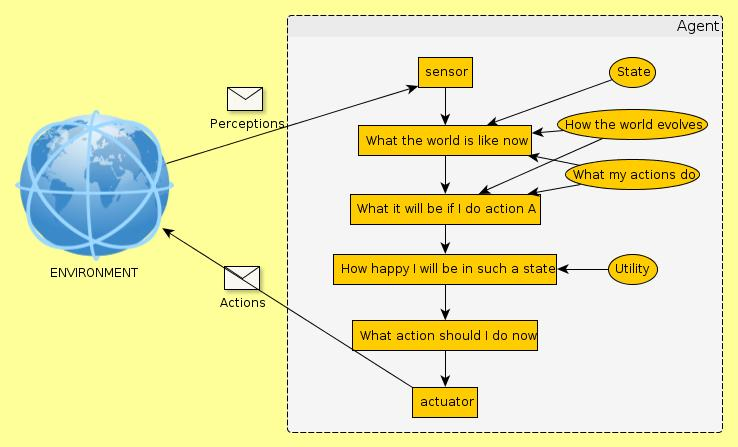
\includegraphics[width=80mm,keepaspectratio=true]{figures/utilityAgent.jpg}}
		\caption{Utility Based Agent Architecture}
		%by RussellNorvig \cite{RussellNorvig}}
		\label{fig:utilityAgent_label}
		\end{figure}


		%%Uncertainty(chap13 Russell... maybe ch16)
		A pure logical agent can find a cul-de-sac on its deductions if the possible contingencies overcome
		the reasoning to deduce the actions to fulfill the goal. These issues are what is called
		\textbf{uncertainty}. Uncertainty is the term used when there are many solutions that lead to the
		goal or if the goal is something not sure to be achieved and the agent faces a choice with no 
		success ensured. 

		For instance, considering a hunter agent in a social simulation of ancient societies, a hunt action
		can be affected by many issues. First you must make a guess about where the preys are. Once you 
		begin the hunting session many things could happen: a weather incident that changes prey grace
		behaviour, other hunters appear to hunt the preys, or dangerous roaming predators. The pure bivalued
		logic agent cannot predict the setbacks so cannot deduce the sucess of the action, and the hunt 
		action will not be launched leading to starvation. If all the logical paths towards the achievement 
		of the goal are troubled by contingencies, the agent could fall in a loop of inactivity.\\ 
		When perfect solution is perhaps non achievable, the agent should be allowed to satisfy the goals
		through a non perfect solution. The decission engine should be changed to accept failable solutions 
		for its goal seeking. Another hunt area should be eligible in the decission process. But maybe,
		although the other area is free of contingencies, it cannot offer a good outcome because is almost
		dessertic. Someway the agent should express a \textbf{preference} and deduce the action planning
		according to it. Preference over the outcomes of and action in the goal seeking activities of the 
		agent encompass the modelling of success probability and benefit quantification. A particular outcome
		should be the fact that the hunter returned home without getting injured and a certain amount of 
		Kg. of meat. 

		\textbf{Utility theory} is used to represent and reason with preferences. Utility theory says that
		every state has a degree of usefulness, or utility, to an agent and that the agent will prefer 
		states with higher utility \cite{RussellNorvig}. Preference and similar issues are modelled through
		\textbf{utility functions}. 
			\begin{equation}
			 u\ :\ E \rightarrow \ \mathbb{R}
			\end{equation}
		Utility functions map desired states to a quantitative dimension, a scoring. Utility ponderation 
		allows to break ties in sub-goal selection. Utility functions will give extra heuristic information
		about the likelihood achieving a goal. If the hunter agent has acces to two areas of hunting, $valley$
		and $wood$ and is more likely to find dangerous predators in the $wood$ although the same preys can 
		be found on both areas, the utility function would assign greater utility to the $valley$. Utility
 		provides a way in which the likelihood of success can be weighted against the importance of the goals.\\
		Preferences, as expressed with utility functions, are combined with probabilities in the general 
		theory of rational decisions called \textbf{decision theory}: \cite{RussellNorvig}
			\begin{equation}
			Decision\ theory = probability\ theory\ +\ utility\ theory .
			\end{equation}

		Utility-based agents are rational and follow the principle of \textbf{Maximum Expected Utility (MEU)}: 
		\textit{An agent is \textbf{rational} if and only if it chooses the action that yields the highest
		expected utility, averaged over all the possible outcomes of the action.}\cite{RussellNorvig}.
		This feature is interesting due to its fit in the Rational Choice Theory \cite{rationalchoicetheo} which tries to give a frame for the explanation of behaviours and decisions in an economical domain.
		It is one of the justifications of using planning strategies in the agents we have developt.
		%TODO a la section de MDP fes una refer\`encia cap aqui
		%\item[Utility and Planning]
		%utility functions applied to runs... 
		%%TODO (Explicar-ho? o es fa al capitol del MDP)

	\end{description}


	%\item Hybrid Architectures 
	%say you can mix everything
		
\end{description}


%%TODO TOASK Differences between Agents & Expert Systems pg17
%% why did we choose agents? why not embed and ExpSyst in our agents?

%%TODO TOASK BDIs? not decided yet. Responc aixo a la part d'agents dins l'ABM?


%%%%%%%%%%%%%%%%%%%%%%%%%%%%%%%

\paragraph{Environment Features}

The design of the agent is conditionated by what is considered ``the environment'' in the real system to model.
It will facilitate or constraint the features and decisions in the development of the agent. Next, some common features that will guide in the characterization of the environment are enumerated \cite[section 2.3]{RussellNorvig}.

\begin{description} 
	\item [Accessible vs Inaccessible] An accessible environment is one in which the agent
		can obtain complete, accurate, up-to-date information about the environment’s state.
		Most moderately complex environments (including, for example, the everyday physical 
		world) are inaccessible.\\
		The more accessible an environment is, the simpler it is to build agents to operate in it.
		Accuracy and completeness about information retrieved is key to decission making.
		All the missing stretch must be supplied with uncertainty managing techniques.
	\item [Deterministic vs non-Deterministic] As we have already mentioned, a deterministic
		environment is one in which any action has a single guaranteed effect — there is no 
		uncertainty about the state that will result from performing an action.
		The physical world can to all intents and purposes be regarded as non-deterministic.
		Non-deterministic environments present greater problems for the agent designer.
	\item [Episodic vs non-Episodic] In an episodic environment, the performance of an
		agent is dependent on a number of discrete episodes, with no link between the performance
		of an agent in different scenarios. Episodic environments are simpler from the agent
		developer’s perspective because the agent can decide what action to perform based only 
		on the current episode — it need not reason about the interactions between this and future 
		episodes.
	\item [Static vs Dynamic] A static environment is one that can be assumed to remain unchanged 
		except by the performance of actions by the agent. A dynamic environment is one that has 
		other processes operating on it, and which hence changes in ways beyond the agent’s control.
		The physical world is a highly dynamic environment.
	\item [Discrete vs Continuous] An environment is discrete if there are a fixed, finite
		number of actions and percepts in it. Russell and Norvig give a chess game as 
		an example of a discrete environment, and taxi driving as an example of a continuous one.
\end{description}

	\begin{table}[h]
	\centering
	\begin{tabular}{||l|l|l|l|l|l|l|l||}
		\hline
		\hline
		\textbf{Task} \textbf{Environment} & \textbf{Observable} & \textbf{Deterministic} & \textbf{Episodic} & \textbf{Static} & \textbf{Discrete} & \textbf{Agents}\\
		\hline
		Crossword puzzle 	& Fully & Deterministic & Sequential & Static & Discrete & Single	\\ \hline
		Chess with a clock	& Fully & Strategic     & Sequential & Semi   & Discrete & Multi	\\ \hline
		Poker			& Partially & Stochastic & Sequential & Static & Discrete & Multi	\\ \hline
		Backgammon		& Fully & Stochastic    & Sequential & Static & Discrete & Multi	\\ \hline
		Taxi driving		& Partially & Stochastic & Sequential & Dynamic & Continuons & Multi	\\ \hline
		Medical diagnosis	& Partially & Stochastic & Sequential & Dynamic & Continuous & Single	\\ \hline
		Image-analysis		& Fully	& Deterministic & Episodic & Semi & Continuous & Single 	\\ \hline
		Part-picking robot	& Partially & Stochastic & Episodic & Dynamic & Continuous & Single	\\ \hline
		Refinery controller	& Partially & Stochastic & Sequential & Dynamic & Continuous & Single	\\ \hline
		Interactive English tutor & Partially & Stochastic & Sequential & Dynamic & Discrete & Multi	\\ \hline
		\hline
	\end{tabular}
	\caption{Examples of task environments and their characteristics.}
	\label{tab:EvironmentCharactExamples}
	\end{table}

%%%%%%%%%%%%%%%%%%%%%%%%%%
%TODO quan parlis de les platforms, FIPA &Co, justifica que anem amb Pandora+ODD. Per paralelisme a MN?
%%%%%%%%%%%%%%%%%%%%%%%%%%


%Features:
%\\
%		  agents ( els features isolats )
%		    goal planning/seeking
%		    reasoning
%		    adaptation
%		    decission making
%		  social interaction
%		  emergence
%\\		    
%		  bottom-up modelization
%		    identify reasoning/deciding units : what will become agents
%		    identify agents' relationships. 
%\\
%		  natural correspondence/matching of identified entities in social systems vs 
%		  agents in the ABMs theoretical framework
%\\
%		  temporal correlation - histeresis
%\\
%%%%%%%%%%%%%%%

\subsection{Complex Systems}

Complexity is a discipline that studies systems that cannot be studied through the analisys of its
parts and the simple composition of those analisys. Usually, \textbf{reductionism} has coped with complicated systems
where the supression of constituents does not change the main trend of its behaviour, and it is used to
work with simplified questions. Let's think for instance in a car which more or less keeps running although 
you remove its seats, the doors, and the lights, to mention some. That is what could be called a complicated 
system \cite{MillerPage2007}.
There are systems where the interrelationship is so rich that supression of one part dismembers all the coherence
of the system. Taking again the car exemple, if we think about the engine, the suppression of a most tiny
gear will change the things, everything will stop. Historically, those systems have been an issue that was 
of concern to many disciplines, Economics, Physics and Biological sciences, that gave arise through an
interdisciplinary effort to complexity science \footnote{here we are not talking about the computational
concept of algorithm complexity.}  \cite{MelanieMitchell2009}. 
Complex science tries to find out how the interactions of a set of constituents build a system that exhibits 
adaptive traits, descentralized organization, and macroscale behaviour patterns.\\

One of the most known systems studied by its complexity are ant colonies. The colony is formed by a limited range
of roles, a queen, soldiers and workers/explorers. Each role exhibits a limited spectrum of behaviours activated by pheromones or stimulus from the environment. Soldiers attack anything that moves non impregnated by the odor of the nest. Unloaded workers follow explorer's pheromons. When food is found a worker returns home. Dead bodies or garbage found are put near other garbage, generating dump patterns. More or less this is the program of ants. And this executed by a huge amount of ants produces an ant colony that manages food resources, reproduction and care, defense and many
other adaptations to the wild life in the forest. It can loose part of its population, can balance workload, a same specific individual group of ants is not needed for an especific task. The colony is ductile, malleable. The ant 
colony acts has a whole with very rich global behaviours. That is a complex system.\\

%TODO exemples : swarm, ecosystems, weather,Belousov-Zhabotinsky reaction, real economic systems, markets
%TODO game of life, we give the pressence of entitty to patterns arising from cell behaviour.

Researchers observed that woods under a fire dissappear at different rates not completely dependent to the intensity
of the focus, nor the climatic conditions. It was observed that under some tree topologies and certain wood
density a small change in the number of trees would mean sometimes the complete combustion of all the wood, and
other times the wood would only burn in a small controlled area. This topology dependant condition is called
\textbf{percolation}. It arises from the spatial relationship between the trees. Considering an ideal situation
where topology protects the wood from percolation appearance, slight changes in some trees distribution will make
them sensible to fire, but the rest of the wood will not burn. These conditions are an example of robustness
in complex systems. But enough changes will collapse it.\\
The strong relationships that give arise to the complex phenomena act as the glue that holds the system, it gives
reason to the system existence.\\ 
Percolation was not discovered studying one tree. It was detected taking into account the whole of the wood and the feedback versus the individual trees.\\

\begin{figure}[h!]
\centering
\setlength\fboxsep{0pt}
\setlength\fboxrule{0.5pt}
\fbox{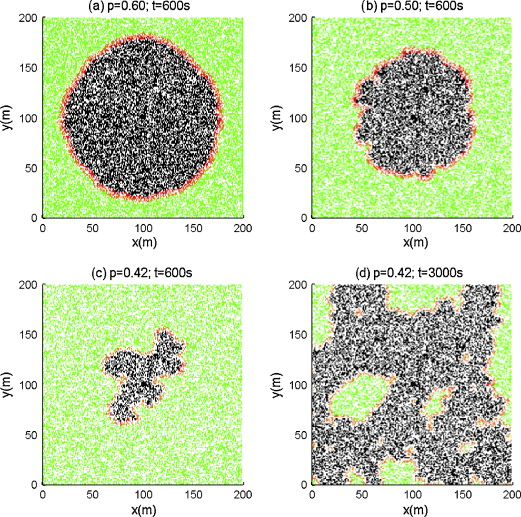
\includegraphics[width=45mm,keepaspectratio=true]{figures/percolation_1.jpg}}
\caption{ Percolation phenomena in fire spreading.}
\label{fig:percolation_1}
\end{figure}

Indeed we observe that there is a system due to the pressence of the macro phenomena. It is the evidence that
something is happening there that relates the constituents.\\

\begin{figure}[h]
\centering
\setlength\fboxsep{0pt}
\setlength\fboxrule{0.5pt}
\fbox{
\includegraphics[width=40mm,keepaspectratio=true]{figures/dictyo_2.jpg}}
\caption{ Development of spiral waves after hydrodynamic breaking of a concentric wave (Zhabotinsky and Zaikin, 1971).}
\label{fig:ZhaboZaikin_1}
\end{figure}


%TODO
%Just as an anecdotic remark, the word ``complex'' comes from the latin word ``plectere'' which means ``to weave'', ``to enwine''.

%TODO exemples : swarm, ecosystems, weather,Belousov-Zhabotinsky reaction, real economic systems, markets
%TODO game of life, we give the pressence of entitty to patterns arising from cell behaviour.
%TODO we see a shape move, form give life to a macro entity, and we observe a lifecycle of operations :
%TODO space translation, shape transformation, appearance, disappearance

%TODO Complex : emergence, self organizing, adaptive, descentralized 

Just to give a compact definition from Melanie Mitchel \cite{MelanieMitchell2009}, ``a complex system is a system in
which large networks of components with no central control and simple rules of operation give rise to complex collective behaviour, sophisticated information processing, and adaptation via learning or evolution. Sumarizing, a complex system exhibits nontrivial emergent and self-organizing behaviors''.

%exemple -> analitzar-lo i posar de manifest la complexitat ???
% and then state what comes next:
The laws that describe its behaviour are qualitatively different from those that govern its individual units.
The advances of computational techniques for scientific discovering is changing the way we confront the models 
and the manipulation of these issues. Computers have allowed new ways of learning about them. Computational techniques 
allow the modelling of many constituents and its relationships, how they assemble to a whole system. It allows us 
to understand and play with the experimental manipulation of the behaviour in a easier way. Computers not only help 
us in studying the surface of the behavioral phenomena but also the internals of complex systems giving insight 
to our explanations and deductions. Besides, computational experimentation has the advantage of controlling the trace 
and generating rich databases of events for posterior analyses \cite{Vicsek2002}.

%TODO ara lligues Complex amb Emergence i pots passar al següent punt
Complex behaviour is tied to a non central global decission process. But, on the other hand, the emerged pattern is
something that does not belongs to a identifiable constituent. It is build from the descentralized dynamic of all 
the constituents. That feature is called \textbf{emergence}.

\subsection{Emergence}


%Emergence is „the arising of novel and coherent structures, patterns and properties during the process of self-organization in complex systems." (Corning, 2002; Goldstein, 1999)

Emergence is a phenomenon where aggregation of individual and local behaviours are the direct cause
of a higher level pattern or global behaviour. Emergence is one of the key concepts from Complexity 
that is studied in Social Simulation. Indeed, emergence is one of the main features exhibited by 
complex systems.\cite{MillerPage2007}
%TODO elabora. Emergence es un key concept

Although we can give features and descriptions, emergence cannot be fully specified due to the vague 
concepts of ``surprising'' and non deducibility \cite{Holland1997} . But some signals can 
be enumerated to circle the concept of emergence. 

A phenomenon will be considered emergent when it is repeatable and surprising, non deducible from lower 
level rules and the relationships of basic constituents of the system.
Emergence cannot be predicted, given our current means, from only the constituents and their addition, 
following the reverse way of reductionism. Reductionism is one of paradigms of science. A system is observed
to detect differentiated parts. Then each part is analized to extract its behaviour. Reductionism states
that the behaviour of the system can be understood from the constituents specifications plus a simple or 
direct aggregation step. This idea can be applied recursively on the same constituents till some atomic element
considered the bottom of the process. The thing is that due to nonlinear relationships, following the inverse
path to reconstruct a sense for the whole system is practically impossible.\\

Even a small and simple set of rules can make a dynamic system generate emergent phenomena. 
If these rules induce non linear relationships the proportion of a perturbation in the system will not 
be paired with the response of it. To use an uninventive example, nonlinear emergence occurs when someone 
\textbf{calmly} says “fire” in a crowded room and produces \textbf{explosive} panic. Unpredictable results 
arise from constituents interactions. It is here where emergence can appear. When a pattern is recognizable 
and repeats usually along experiments, is plausible to be considered emergent \cite{Holland1997}.\\  

There is potential for emergent phenomena, i.e., when: 
\begin{itemize}
 \item Agent behaviour is non linear ( weight sum of variables), or is expressed with discontinuities, if-then rules in a categorical framework or in discrete non continous manner.
 \item Under memory phenomena, path-dependence, and hysteresis, non-markovian behavior, or temporal correlations, including learning and adaptation. 
 \item Heterogeneous interactions between agents.
 \item When there is unstability to perturbations although the system could be defined linearly.
\end{itemize}


\subsection{Evolution}
%TODO\underline{	Darwinisme : survival of the fittest.
%		Ingredient afegit per a testejar l'adaptabilitat i el fitness de les dues estrategies : HG vs AP
%		Dins el mark evolutiu establirem la competencia entre les dues estrategies : qui pugui tenir una
%		millor supervivencia del seu offspring perpetuara  la seva estrategia (ADN)
%		}

Evolution theory is the result of observations along several years made by Charles Darwin in his trips to Galapagos Islands and the study of native species of finche birds. 

\pdfcomment{Home és força més complicat eh...si de cas digues que Darwin va començar a formular-la a partir de les nombroses observacions fetes en un viatge de varios anys, etc.}. 
\\
\pdfcomment{ATM:done?}
Darwin proposed that the varieties and specializations of observed species was imposed by the topology of the 
island and the local conditions of each one. The theory arised from the following points in conjunction of the observations. He based his deductions on the next hypothesis:
\begin{itemize}
	\item Gradual change over long periods can produce very large effects.
	\item Population growth combined with limited resources creates a struggle for
	existence. 
	\item Collections of individuals acting in self-interested ways produce
	global benefit. 
	\item Life seems to allow almost infinite variation, and a species’
	particular traits seem designed for the very environment in which the species
	lives. 
	\item Species branch out from common ancestors.
\end{itemize}

Darwin called \textbf{Evolution by Natural Selection} to the improvement by mutation and competition process 
where individual beings produce offspring at a rate greater of the survival rate ( otherwise they 
would extinct). The offspring is almost equal to the parents except from slight variations. At 
some point the population will saturate the niche and they will compete for the resources.\pdfcomment{ATM:busco ref}
The more adapted individuals are considered those who will satisfy their resource needs and
have higher reproduction success. This will imply that a great number of offspring that inherited
features from their successful parents will populate the environment. These traits will persist
through the time from generation to generation. This would explain why individuals are as they are
and not other way. Adaptation comes from the small perturbations or changes between parents and
offspring. This is an open door to the appearance of an improved trait that would increase the adaptation
of the new generation. Hence, change after change the Evolution sculpts step by step the organic beings
making them more adapted to the environment. Traits that does not allow to survive nor reproduce will 
not appear in the next generation, except due to some rare mutation but that will be purged again in the 
competition game against the environment.\\

To summarize the major ideas of Darwin’s theory:
\begin{itemize}
	\item Evolution has occurred; that is, all species descend from a common
	ancestor. The history of life is a branching tree of species.
	\item Natural selection occurs when the number of births is greater than
	existing resources can support so that individuals undergo
	competition for resources.
	\item Traits of organisms are inherited with variation. The variation is in
	some sense random—that is, there is no force or bias leading to
	variations that increase fitness. Variations that turn out to be adaptive in 
	the current environment are likely to be selected, meaning that organisms with 
	those variations are more likely to survive and thus pass on the new traits to their
	offspring, causing the number of organisms with those traits to increase over 
	subsequent generations.
	\item Evolutionary change is constant and gradual via the accumulation of
	small, favorable variations.
\end{itemize}

Darwin theory had some points to be clarified. How did parents pass their traits to the offspring?
The process of refining these theories comprised the addition of Mendel's theories lasting till 
the past century where everything was unified with the descovering of DNA and genomics. DNA is the 
way in which are encoded the traits that the organic being will probably exhibit in his life, and 
also DNA is the transmission medium of the traits in the reproduction process. We will take \textbf{Richard Dawkins} 
position as our final work metaphor for evolution and natural selection\cite{Dawkins1990}.\\ 
As it is mentioned, part of the working framework of our simulation is based on the ideas of evolution and ``natural selection''. We understand ``natural selection'' as a process that "rewards" adaptive solutions and penalizes those less adapted. Darwinian Evolution is the result of the continued application of this screening and the persistence of adaptive patterns and what comes off of them. Persistence is produced through the reproductive process of agents. Regularly an agent generates a copy of itself with some disturbance in their features and takes charge of it for a period of time. The extraction capacity of system resources, adaptability,  marks their survival and that of their offspring. If the offspring survives, the configuration is maintained over time and gets another chance to be perpetuated when this new generation begets his sons / daughters. We use evolution as a tool for selection of configurations to respond more adaptively than others, working with the hypothesis that selected ones would correspond to reality. We simulate systems plus the evolutionary process. Our utility functions, birth \& mortality are filters to keep or remove agents of the system depending on its performance against its lifecycle.\\ 
We are applying a parallelism between DNA information and configuration or features in the agent. The features stablish
the policy of the agent. For instance, the Gujarat project would differentiate between HunterGatherer way of living from AgroPastoralist way of living through this features.
\pdfcomment{Caldria que, abans de començar a enumerar tots aquests conceptes, la secció "Conceptual Framework" tingués un paràgraf explicant el que es trobarà el lector a continuació. Si no, queda com raro perquè són conceptes molt diferents}
\\ \pdfcomment{ATM:done}
\paragraph{Coevolution}
%TODO \underline{	Dos grups responent al medi. Pressio Evolutiva. El que fa un afecta a l'altre, aixo provoca una
%		resposta d'adaptabilitat. Estudiem el feedback evolutiu entre HG,AP, i medi.
%		Close interrelationship, strong feedback. It is an environment prone to emergent patterns.
%		}

\textit{When two or more species form an interdependent ecosystem the evolutionary progress of part of the ecosystem will generally induce co-evolutionary changes also in the other species} \cite[p.154]{Gross2008}.

Long ago, bacteria and plancton dominated the seas. There was only microscopic life. Then appeared photonsynthesis
based microbes. With Sun light and CO$_2$ chemistry they spread at a greater rate than their neighbours. Photosynthesis
microbes filling the seas plus millennia produced the oxygen filled atmosphere of the planet. Changes in the atmosphere
changed weather and many other chemical properties in the planet. The atmosphere contained ozone which barred the 
UV rays of the Sun which forbidded life in the surface. Then some individuals appeared with capabilities to get out of 
the water and breath the air of the surface. It is an example of mutual feedback between the environment and the evolving 
life beings. But this feedback can also happen between these beings, and then it is called coevolution\cite{Dawkins1990}.
When the adaptive process of an species produces a change that motivates selection of new adapting traits in other
species which in turn affects the same way the first species we have coevolution. For instance, the relationship 
between a prey and a predator will induce coevolution. The hunting activities produce death in the prey species, hence
motivating the selection of traits that give more probabilities in front of a predator attack. Predators feast on preys 
with feble traits. Old feble traits dissappear. Then predators must hunt the individuals without the feble traits. Incompetent predators will starve and a new elite will appear. A mutual selection pression is stablished between both species feeding changes of new ``attacks'' and ``counterattacks'' and ``counterattacks'' to the ``counterattacks''.\\

Although we will not wire explicitly coevolution in the two studied social models we expect to see this phenomena. Sugarscape will be the framework for the competition between classical Sugarscape agents and sophisticated-AI ones. In Gujarat project we expect to observe coevolution between HunterGatherers and AgroPastoralist as they compete for resources and land. The cultural traits are considered an analogy of adaptive strategies. 


\paragraph{Cultural Evolution}

%The ideas from Evolution have been adapted to study the sociocultural dynamics in human society... blabla  \textbf{cultural evolution}.
%%TODO 
\pdfcomment{ATM:posa abstract de resilience de Montpellier}
Behavioural Sciences trying to explain the cultural idiosyncrasy of human beings have traced a parallelism between its dynamics and Darwinian Evolution theories. Cultural Evolution \cite[ch11.]{Dawkins1990}\cite{Stanford_CultEvol}( socio-cultural evolution, CE ) states an analogy with the selection, adaptation and innovation processes descrived in the theories of darwinian evolution. Culture endows humans with a mental frame of assumptions and behaviours that affect their response to the environment. This has an impact in human performance to the treats of the environment and hence adaptation to it. Culture is a trait that like the physical features that conforms an individual will be crutial to its ressilience.\\ 
Another important dimension of culture is transmission. Culture like genes is something parents can transfer to their offspring. Also, besides receiving a vertical endowment from parents, culture can also be adquired from other peers in a oblique way, maybe from brothers and sisters, or grandparents. This process is called cultural transmission. Just happens like in replication of parental genes, there exists the possibility of errors in the copy process. Either the communicator of cultural traits or the receiver can alter the information leading to errors or improvements. There could exist also improvement in knowledge due to revision and update of the results of the behaviours through experience. Next a table is presented to show the paralelisms between evolution theory and cultural evolution theory.

	\begin{table}[ht!]
	\centering
	\begin{tabular}{|p{7cm}|p{7cm}|}
		\hline
		\textbf{Modern Evolution Theory} ( NeoDarwinism )
		&
		\textbf{Cultural Evolution}\\
		\hline
		Information is encoded in DNA strands, chains of genes, the genome. It will be expressed in the physiological traits, structure and metabolism, the phenotype.
		&
		The cultural corpus, containing ideas, mental frames, patterns and know-how, is added to the behaviour of the individual.\\
		\hline
		The physiological traits achieve some level of fitness to the environment setting the adaptability and ressilience of the individual.
		&
		Behaviour and know-how conditions the response  and adaptability to environment(physical world and other entities) challenges. How well the individual responses defines its fitness and ressilience.\\
		\hline
		Higher ressilience gives higher oportunities for offspring generation. The fittest individual retrieves more resources and avoids best the treats. The fittest reproduces more.
		&
		The individual endowed with a culture that enhances its ressilience survives to transfer it to its offspring / partners / peers. Higher ressilience gives higher oportunities for offspring generation. The fittest individual retrieves more resources and avoids best the treats. The fittest reproduces more.\\
		\hline
		Parents transfer their gene information to offspring : vertical transmission.
		&
		Cultural transference can happen through multiple channels, parents, peers, authorities : oblique transmission.\\	
		\hline
		Copying dna although it is a process with correction mechanism has a ratio of error that introduces mutations in the copy and hence new information that entails new traits, which can report benefit or lead the individual to a lesser fitness than its parents.
		&
		Learning is a process where the absorved corpus can be altered by the comunicator, the receiver, or due to added new knowledge. The error in transference or execution of learned skills and knowledge can lead to innovation.\\
		\hline
		Offspring inherits traits. There is a correlation of parents' fitness respect offspring's fitness. Usually , strong parents produce strong offspring which will find easier to develop in the environment and hence reproduce, repeating the process from generation to generation.
		&
		The individual endowed with a culture that enhances its ressilience survives to transfer it to its offspring, partners or peers. The individual acts as the medium through which culture is transferred.\\ 
		\hline
		Fit gene combinations persist in time displacing less adapted ones.
		&
		Fit culture or knowledge persists in time displacing less adapted ones.\\		
		\hline
	\end{tabular}
	\caption{Summary of parallelisms between contemporary evolution theory and cultural evolution theory.}
	\label{tab:EvolThVSCultevol}
	\end{table}

CE theory assumes a morphism with contemporary evolutionary theory; CE theory states that the current state of culture for some social group is a result of natural selection upon the individuals exhibiting some cultural traits that changes its ressilience in the environment. Environment preassure will be a selection and scanning mechanism of cultural traits.

Applying these ideas, concerning the Gujarat project, we will try to explain the change from one adaptation strategy of hunter and gathering to an agropastoralist one based on the assumptions of selection and ressilience applied to both strategies. 

%TODO
%ara justifica que CE et fa la seleccio etc etc...

%in gujarat : CE as a frame of selection process to find the enviromental conditions that
%allow equilibrium between HG \& AP and the conditions that would trigger the extinction of
%HG way of life.
%Produce the steep process for the transition from one strategy to another

We study the skills and strategies for resource exploitation. The successful strategy, hunting and gathering versus agropastoralist activities or sophisticated AI versus classical agent, will yield a greater probabilty of success to the agent. The evolutive-coevolutive framework will trigger a dynamic of selection and gradual change. In the long term we will observe the equilibrium properties reached by coevolution. 

%%TODO 
%For Sugarscape we think sophisticated agents will overcome classical ones, but for Gujarat our aim is to reach the coevolution results that lead to a equilibrium of the two adaptive strategies.\pdfcomment{Coevolution és un concepte lligat a Evolution, no a banda. A més, caldria que parlessis sobre el concepte d'evolució cultural, perquè si no, és difícil entendre per quin motiu volem aplicar-ho a simulació social} \\ \pdfcomment{ATM:done} 

In our study of transition from HG to AP, both groups will be modelled as two different typologies of agents. Each typology will account as a differentiated group where members will belong to it along all their lifes. When an agent emancipates from its parents takes the decision of being HG or AP according to an evaluation of which of both groups seems more succesful. When an agent takes the same role of the parents it can be seen as vertical transmission of cultural traits. When an agent takes a role different from the parents we can assume that it learned these skills from neighbours in environment. It must be stressed that we pay attention to transition to agriculture, not to emergence of agriculture in a only HG environment. Somehow agropastoralist yet exists in the environment. We only want to know how different environmental conditions favor one or another strategy and why HG kept being a plausible strategy in Gujarat when it had dissappeared in other places.
Each group has particular actions representing their way of making their living. HG execute Forage actions and AP execute Crop actions ( with subtasks of preparing, cropping and harvesting fields ). But there societies where both strategies coexists inside a group. Individuals show competence and skills to survive applying a mix of HG and AP actions. So the final aim is to remove groups. If we understand strategies as knowledge, knowledge will be contained in the agents in a fuzzy and dynamic way instead of wired elegible actions. There will be mixed agents that will execute HG actions and AP actions with different proficiency on them. We will call \emph{skills} to this construct. And these skills represent the ''genetic'' traits that we want observe evolving from this framework of CE. Each agent will have proficiency in the four skills from the merge of HG and AP groups : hunter, gather, crop, shepperd. A typical Hunter Gatherer considered in the scope of this master-thesis work would be an individual with a near 100\% proficiency in hunting and gathering while having 0\% on the other actions. And a pure AP individual would be endowed with the complementary asignation, 0\% for hunting and gathering with almost 100\% for actions Crop and Shepperd\ref{fig:SkillProfiles}. In the long term we want to observe the gradual transformation from one strategy to another through the change of profiles of proficiency. As knowledge is something where skills are not mutually exclusive, we consider reasonable that agents can execute the same set of actions. The dynamics of selection and environment preassure will benefit some configurations from others. This can lead to profile attractors or cyclic emergence of profile patterns according to the periodicity of climatic fluctuations.


\begin{figure}[h]
\centering
\setlength\fboxsep{0pt}
\setlength\fboxrule{0.5pt}
\fbox{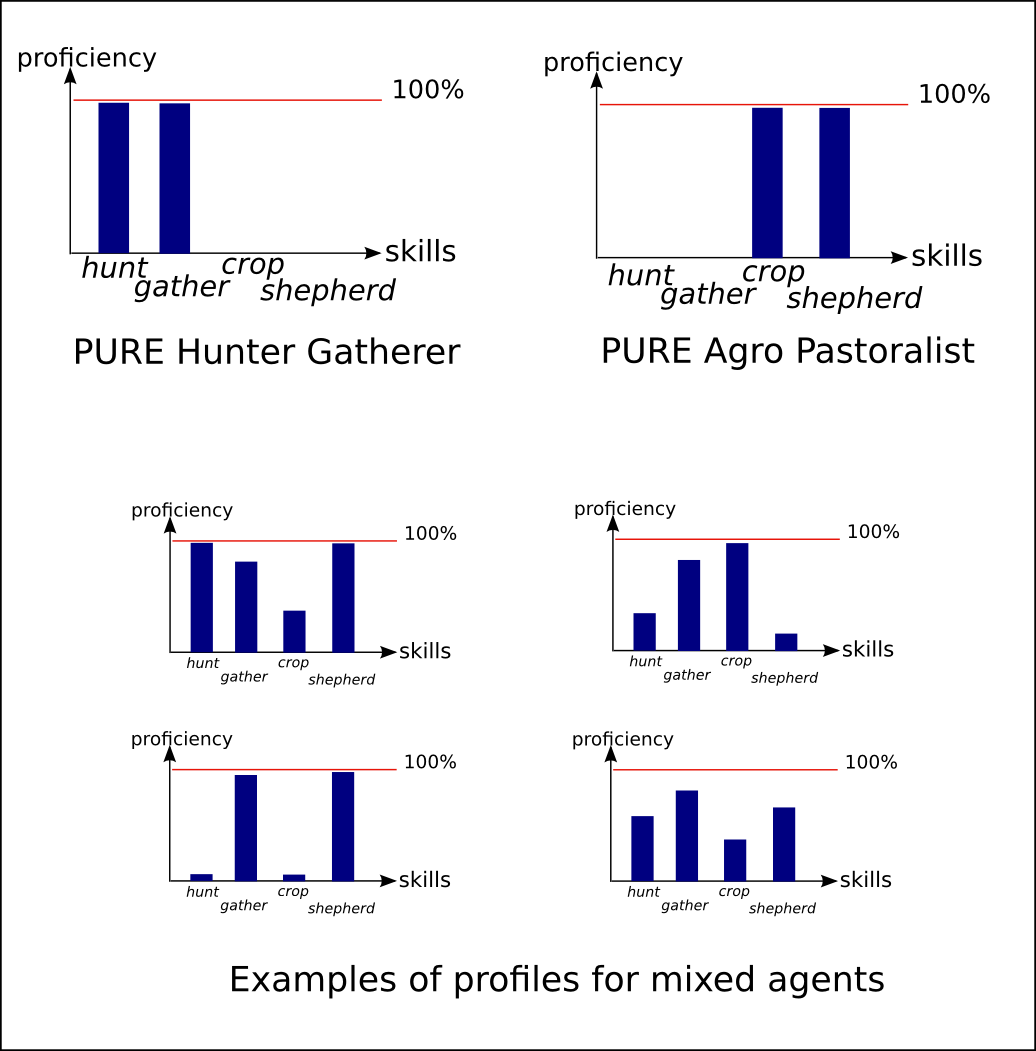
\includegraphics[width=120mm,keepaspectratio=true]{figures/skillProfiles.png}}
\caption{Skill Profiles.}
\label{fig:SkillProfiles}
\end{figure}


\chapter{Gujarat}

\section{Introduction}

This chapter exposes the work in case study one in the Simulpast project. 
The text follows the structure of ODD documents we have been using to register our decisions and models and as a comunication report in the group. ODD is a document structure with an overall look of high-level specification but open to detailed explanations \cite{GrimmBergerODD2012}. ODD documents have been thought to be able to yield enough details so another researcher can replicate the system and produce the same results and conclussions. We think this feature is a good point for expert-modeler communication. It helps to keep an account of the details and the refinement of the discursive part of knowledge from social science experts into formal components of the model. We know there are more sophisticated protocols to guide the design of an agent system (KAZ... )\pdfcomment{ATM:llistar i referenciar}, but we wanted to ensure the communication part for ellicitation applying ODD phylosophy following a growing procedure of a seed system based in Sugarscape \cite{EpsteinAxtell}.

%TODO en algun punt parla d'AUML. perque no l'usem. La interactio agent-agent no es basa en un llenguatge ni
% cap transferencia estructurada complexa, nomes els tokes d'informacio de recursos. NO HI HA DIALEG 

%TODO que fem nomes HG enlloc de HG+AP es diu a la intro de la tesina
%%Centrat en HG encara que es donen detalls dels AP que s'estan afegint en la versi\'o actual.

%TODO the chapter dresses the main ODD structure with extra explanations extending its technical scope. The aim is not only to comunicate a model but the ``path''  that leads to it. <--- pero no ho tens ja aixo amb l'ODD??? 


The first section of the chapter introduces the observations and hypothesis of archeologists that have been studying the scenario of Gujarat during the transition and settlement of agriculture. This part states the motivation that leads to the purpose of the model. The following sections get deep in the details of the system, enviromental features, resources, weather conditions and dynamics, the agents and the features for matching the relevant system dynamics to solve the question. After the modeling details the next section exposes the solution for solving the decision making of the agents. A planning strategy is needed to achieve maximum adaptability of the agents under the different weather conditions scenarios for stress experiments. Markov Decision Processes and UCT algorithm will be introduced. Once the decision making is explained, different solutions are presented to enhance efficiency and throughput of steps per second in the simulation. The last sections cover the experimental part of the project. It will be centered about the ressilience of the current social group modeled, hunter gatherers. %TODO posa una mica mes

%%1.-target - purpose

%%2.-model details and components following ODD guidelines ...

%%TODO esta ben colocat??
%%3.-information sharing : es part de la interaccio agent-agent,pero tambe un apartat cientific del model

%%4.-decision making

%%5.- the efficiency issue

%%6.-results

%%7.-discussion

%%8.-future


%dius que parlaras de gujarat a aquest cap\'itol.

%descriuras l'entorn i les caracter\'istiques que es consideraran en el model.
%la descripci\'o est\'a basada l'estructura del document ODD que s'usa en l'equip.

%Enlloc de tenir una guia mes rigurosa y ortodoxa s'ha volgut experimentar amb aquest
%tipus de document per veure si facilitava la comunicacio modelers<->experts.

%ens hem centrat en HG. estem posant en marxa els AP ( posar-ho tambe a un apartat future?)

%parla de l'extraccio de coneixement, la dinamica de reunions i entrevistes, l'ecotono com a 
%procediment de brainstorming i d'introduccio de problem-model que s'ha aplicat
%en altres projectes d'arqueo --> didactica del pensament de modeling per als experts
%i didactica dels conceptes per als modelers


%%TODO
%Smart Agent
	
%	Decision Making :\\
%		stressful environ -> changing rules -> adaptability -> hypoth-deduc
%		we do not have an algebra or HG rules to reason about system dynamic -->
%		--> hypoth-deduc through planning schema --> bandit game --> mdp --> uct
%	Hypoth-Deduct\\
%	--------MDP\\
%	--------UCT\\
%	--------backed by OptForagTheory & RationalChoiceTheory\\
%	--------BSC day!\\
%	-------- ISSUE { other agents actions are not included in the Hypoth-Deduct schema of
%		-------- UCT. the agents spread over the map more or less uniformly.
%		-------- We do not want competition between them, we want fairplay.
%		-------- We want the group dynamic... Some agent will be lucky, some none.}
%	--------rule agent : we do not want fix set of rules\\
%	----------------learn them? from a setting that we will alter\\
%	----------------to induce change???\\
%	----------------we want adaptability. To the current moment, we choose
%			planning\\

%posa que la coevol s'obsevar\`a en els profiles dels skills --> dinamica de
%la profficiency : from HG to AP, oscillations HG<-->AP, HG,AP will be attractors given some
%conditions : detect such conditions 

%efficiency:
%	LR - HR
%	Settlement Areas
%		Introduction of LR decision making displaced these structures
%	MDPState knowledge sharing : ref to knowledge
%	Extrapolate (in construction)
	
%results
%	grafiques LRQ vs LR ( al mail ???)
%		you do not have to run more than the bear, just more than your friend
%	ressilience : 50 years
%	information sharing
	

\section{Target Description}

Northern Gujarat is a marginal environment between the Thar Desert and the more fertile area of
Saurashtra. This region is an ecotone, characterized by the seasonal influence of the monsoon where
contrasting ecological niches are in tension and small climatic shifts can generate significant
environmental changes, eventually affecting resource availability. Archaeological evidence points to
the presence and possible coexistence in the area of groups of people with different resource
management strategies and mobility behaviors: hunter-gatherers (HG); agropastoralists (AP).
The aim of this study is to model resource management and decision making among hunter-gatherer
groups in this region to explore adaptive trajectories and performance in relation to a) environmental
variability and b) the appearance of other specialized groups.
What factors play a role in HG persistence or disappearance in arid margins? Is the advent of agro-
pastoral behaviour a big enough change to explain the disappearance of HG behaviour? Does climate
variability affect HG behaviour?
The agent-based simulation here proposed explores the potential for the persistence of hunter-gatherer
(HG) communities relative to climate-driven environmental change during the Holocene in N Gujarat, a
semi-arid region in NW India.


Note:
The modeling workflow is following these steps:
1. Environmental settings and climate engine
2. Resources and energy flow
3. Socio-ecological behaviour of HG
4. Socio-ecological behaviour of AP
5. Cultural transmission

This scaling approach includes three main theoretical and methodological research aspects:
1. Human behavioral ecological approach and socio-ecological co-evolutionary framework
2. Model based vs rule based action planner of the agents
Up to the date, steps 1, 2 and 3 have been developed . Work regarding AP models and cultural
transmission is in progress.



\section{Purpose}
In our starting hypothesis HG groups are adapted to marked seasonality (represented by the
monsoon) in the arid margins of northern Gujarat. We intend to explore HG resilience (Holling 1973,
Carpenter et al. 2001) considering climate variability.

Future : We intend to explore HG resilience considering the appearance of AP

\section{Entities, state variables, scales}


The model is designed to explore separately socio-ecological behaviours of two isolated populations: 1)
Hunter-Gatherers (HG) agents and 2) Agro-Pastoralist (AP) agents. This separate simulation of the
two groups is needed to obtain independent, coherent and consistent models of HG and AP decision
making. Once the dynamics of the modeled systems are understood for each population, agents from
the two populations will be combined in a single simulation execution. These will be considered as
independent groups, and interaction between agents will be limited to other agents belonging to the
same population. But the scope of this work is focused on exploring the socio-ecological behaviour of HG populations.

Agents from one population will interact within a given territory. It is characterised in terms of: a)
geographical information derived (height, slope), and b) landscape (soil types, resources). This
territory and its characteristics will generate an environment that will allow to portray differences in
strategies regarding settlement, mobility and resource use.


\subsection{Scales}
\paragraph{Agent Scale}
The basic agent is defined as a couple (one woman and one man). This is considered to be the entity
engaging in all decision-making processes and actions modeled in the simulation.
\paragraph{Time Scale}
Time Scale for the simulation is one day. This time step is coherent with the granularity of agents’
planning. The decision making of HG happens at the level of their daily action.
%%TODO recorda el pas que es va fer de SEASON a DAY... posar la rao perque es va fer 

\paragraph{Space Scale}

The spatial resolution of the proposed simulation model is constrained by the resolution of available
relevant geographic data and the nature of the agent mobility and resource gathering activities being
modeled.
Hence, it was decided to use 31.5m x 31.5m cells, corresponding to ca. 1000 square meters. This is
the level of resolution of the most detailed geographical information available for the area. This surface
fits the type of settlements recognized from archaeological surveys.


\subsection{Environment}
The simulation environment is large enough to develop all potential processes defined by the model according to the
experts' advice. It extends over an area of 50 Km x 50 Km (2500 Km2). Space is represented as a regularly spaced grid
of cells (a raster map). Each cell is a square of 31.5 m per side, and the total size of this environment
translates into a space of 1600 x 1600 cells (50,400 m x 50,400 m).
The ground model includes elevation and land features. Elevation is determined by a Digital Elevation
Model (DEM), a raster map containing the elevation value for each cell calculated from contemporary
satellite imagery. Land characteristics are reduced to three elemental categories:

\begin{enumerate}
\item Water: represents rivers and lakes.
\item Dune: represents the top area of the dune, which can be settled. Home location of the
agent will always be in a dune cell.
\item Interdune: represents the interdune(between water and dune) area where resources grow. The different land
features do not seasonally change in extension but their productivity (in terms of moist content
and therefore resources supported) does.
\end{enumerate}

The cornerstone of our environmental modeling is the climatic 'engine'. The climate module
determines the quantity of rain that precipitates evenly on the landscape on every time step.
Precipitation is used in conjunction with the terrain model to calculate the amount of biomass for each
cell and season. The climate model is based on historical data, as well as Holocene monsoon models.


\subsubsection{Climate}

The focus on resource utilization strategies within a particular environment requires to make explicit
the potential variations in the landscape. In particular for our case study, the presence of the monsoon
generates a strong seasonality (asymmetrical precipitation patterns).
Monsoon seasonality determines the presence of three critical “moments” in simulation time, each
spanning 4 months. Therefore, the seasonal subdivision in three periods will be repeated in a cyclical
way as follows below. Identification of months from western calendar covered by each of the seasons is done 
taking the first letter of the month name and using the concatenation to label the season. So "JJAS" stands 
for the season that covers June, July, August and September, for instance. "ONDJ" is the label for the 
season covering October, November, December, January. "FMAM" is for February March April May.    


\begin{enumerate}
\item JJAS (rain season: high precipitation, high temperature, low evapotranspiration)
\item ONDJ (post-Monsoon: low precipitation, cool temperature, medium evapotranspiration)
\item FMAM (dry season: low precipitation, high temperature, high evapotranspiration)
\end{enumerate}


It is important to note that any given “year” in the model starts with the beginning of the rain season
(June). In fact, virtually all rain in the region is carried by the monsoon that falls between June and
September (JJAS). Therefore, it is during the JJAS season that the totality of the generated yearly
precipitation value is calculated (following a Gamma distribution). No additional precipitation is
considered for the remaining eight months of the year (ONDJ and FMAM).

\subsubsection{Resources}

Each cell has a finite number of resources. Resource availability for each cell is calculated from the
following variables:

\begin{enumerate}
\item Yearly precipitation (rainfall, using a Gamma distribution)
\item Type of cell (Water Body, Interdune, Dune)
\item Mean yearly Biomass per cell and type.
\item Cell history (e.g. whether the cell was used for crop in a previous step or part of the resources
were consumed before).
\end{enumerate}

Resources include the total biomass that can be found in a cell (fauna and flora). They are exploited
by HG agents engaging into foraging activities. Foraging includes activities such as hunting animals
and gathering plants, fruits, seeds, etc. Indeed, from a literature review it is clear that secondary
biomass production (animals) is directly related to primary biomass quantity. Moreover, as there is no
interest in our simulation to explore gender-based labour division we decided to consider hunting and
gathering as a single activity (foraging) without distinguishing between plant or animal utilization. In the
light of this, it was decided to consider a value for cell (dune vs interdune) based on published
information of primary biomass production in desert (dune) and savannah (interdune) biomes (after
Kelly 1983 – Table 3).


\begin{table}[ht!]
\centering	
	\begin{tabular}[c]{|l|l|l|l|l|}
	\hline
	Cell Type & Yearly Primary Biomass Production & Efficiency & Energy & KCal \\
	\hline
	Dune (desert) & $700g/m^2$ & $13\%$ & $1820KJ/m^2$ & $435KCal$ \\ 
	\hline
	Interdune (savanna) & $4000g/m^2$ & $23\%$ & $18400KJ/m^2$ & $4395KCal$ \\
	\hline
	\end{tabular}
	\caption{Parameters for resource parametrisation according to Kelly (1983; Table 3, p. 284).}
	\label{tab:tabResources}
\end{table}

\begin{enumerate}
 \item Cell area = 1000m2
 \item 1 g Primary Biomass = 20KJ
 \item 1 kcal = 4.184 KJ
\end{enumerate}



\paragraph{Distance to water}
This average value of resources is modified based on the distance of a cell from the closest
water body. This weight decreases linearly to the distance, and models the heterogeneity of
biomass generated by a higher presence of flora and fauna near the zones where needed
water can be collected. The update due to resource growing will depend on the matrix of distances
to the nearest water body representing this information.

\paragraph{Efficiency}
The total primary biomass value does not constitute the entire primary biomass available for
consumption to animals and humans. This value represents the entire biomass production
including both edible (fruits, tubers some roots etc.) and non-edible (wood, stems, branches
etc.) parts of the plants. The ratio of profitable biomass versus whole biomass will be the
efficiency value specified in the above table that allow to calculate the energy effectively
available for humans.

\paragraph{Domesticated cell} (work in progress)
The model is prepared to tag cells wether they are domesticated or wild when we will introduce AP 
agents in the runs\pdfcomment{ho deixo aqui o a future work?}. Domesticated plant resources define the density of domesticated plants found inside the cell. It is important to note that wild and domesticated types of resources 
are mutually exclusive: i.e. wild resources are not found on cultivated plots. 

The basic idea for a domestication cell is that of small scale shifting cultivation, in which a plot is
cultivated following a cycle that includes abandonment so to allow soil properties to recover. A
domesticated cell can be planted for a maximum of three consecutive years. It then needs to be
abandoned for a minimum of three years (during which it will be considered as Fallow). After three
years of abandonment the cell becomes wild and can be used again for agriculture. If a plot is
abandoned before being cultivated for three consecutive years it will have to remain abandoned for
the same amount of years it was worked. During these years it will remain fallow, after that it will
become wild again.

Crop cells change temporary their state to Fallow during the FMAM season, where no agricultural
uses can be executed. It turns to Crop again during JJAS season, and will be ready to sow at the end
of it.


\subsection{Agents}
The following attributes have been chosen to account in our model.

\begin{enumerate}
\item[Age] - A numeric variable that keeps track of how many time steps a given agent has been
active in the simulation.
\item[Children] - A collection of human entities. The number of children is bound by resource
availability. Birth and mortality rates depend on resource availability and hence regulate the 
number of children.
\item[Home location] - the cell where the agent resides and the spatial centre of the activities it
carries out. Any number of agents can share a given cell.
\item[Home range] - Maximum distance an agent may travel in one day. This attribute restricts
foraging and social activities from taking place in cells too far from the agent Home location.
The area enclosed in the circle of radius “Home range” is divided in six equal sectors. Such
division models the idea of direction of exploration for the agent actions, while simplifying the
decision-making process (an agent will choose to forage in one of the six sectors,
independently of single cells).
\item[Food needs] - Value that sets the minimum calories a given individual needs in each time step
in order to survive. The total amount of food needs for an agent is computed as the sum of the
food needs of the individuals that form a given agent. The probability of death increases for all
the individuals that form a given agent when this basic quantity of resources is not foraged
within a day (due to starvation). Needs are defined by the following table:
\item[Available forage] - Daily time that an agent can spend on foraging. The total amount of
foraging time for any given agent is computed as the sum of the foraging time of the
individuals that compose it. Foraging time increases from infancy to adult life, modelling
learning processes as defined in the following table:


\end{enumerate}

%%TODO FUTURE

%\item Relationships – These are the connections between agents. The following types of
%relationship are considered:\\
%	\begin{enumerate}
 
%	\item Acquaintance – This is the result of having met at some time in the past. A numeric
%	value is used to track the intensity of the relationship. This value changes with and
%	depends on the actions of the involved agents.\\
%	\item Next Of Kin – Agents connected by family ties (the agents have some common
%	ancestor). The closeness of the family tie is also modelled with an intensity value that
%	remains constant throughout the agent's life. The value is inversely proportional to the
%	distance in the genealogical tree.

%	\end{enumerate}



\begin{figure}[h]
\centering
\setlength\fboxsep{0pt}
\setlength\fboxrule{0.5pt}
\fbox{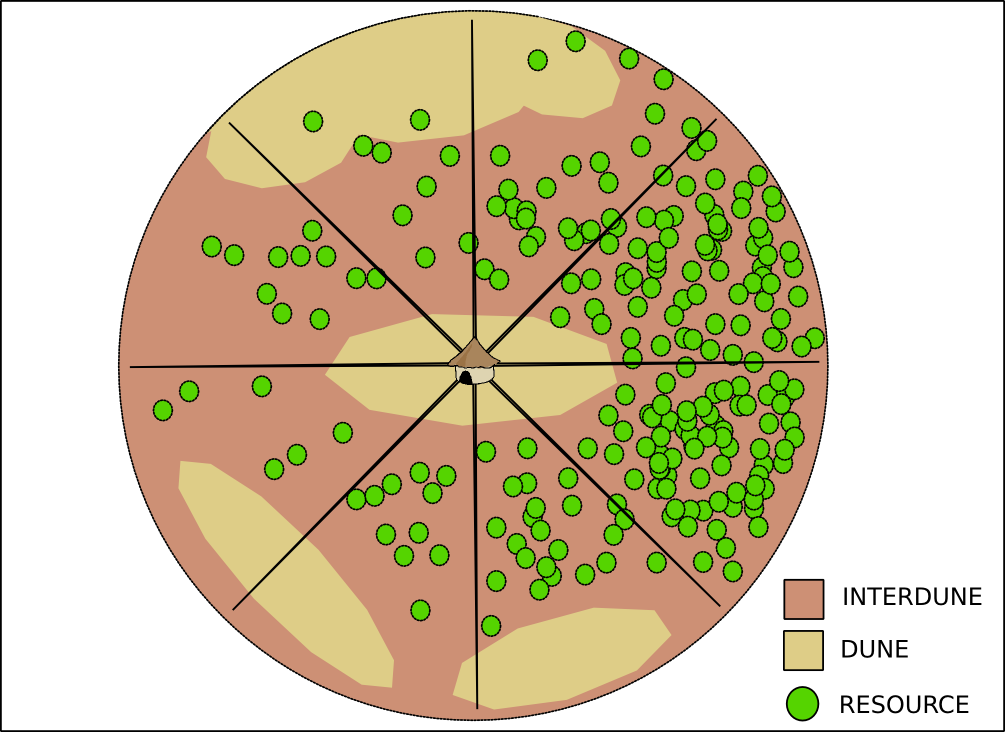
\includegraphics[width=120mm,keepaspectratio=true]{figures/sectors.png}}
\caption{Figure. Home range division for foraging and moving home actions}
\label{fig:sectorsDivision}
\end{figure}


Tables. Individual caloric requirements (left), Individual foraging time (right)

figures pg35 


\section{Process overview and scheduling}

Execution follows two time-scales. On the one hand, three processes (‘yearly precipitation’, ‘biomass
yearly production’ and ‘population size adjustment’) are executed once every year. On the other hand,
agents decision-making processes are updated on a daily base. The simulation follows this schedule,
beginning the first day of the JJAS season:
For each year:
\begin{enumerate}
	\item 1. Precipitation calculation
	\item 2. Biomass yearly production
	\item 3. For each day of the year:
	\begin{enumerate}
		\item a. Daily biomass availability
		\item b. Agent planning:
		\begin{enumerate}
			\item i. Knowledge update
			\item ii. Choice of actions
		\end{enumerate}
		\item c. Execution of agents actions
	\end{enumerate}
	\item 4. Population size adjustment
\end{enumerate}


Details for each simulation phase are given hereafter.


\subsection{Precipitation calculation}
The total amount of rain is calculated as a random number following the Gamma distribution defined in
section 7 (Input Data)
\subsection{Biomass Yearly Production}
The biomass that a cell will produce in an entire year is calculated from rainfall and mean year
production for its particular type, provided by historical records.
We consider a linear relation between rain and biomass production. The deviation of rain in a given
year from the period mean allows interpolating the amount of biomass deviation from the yearly mean
biomass. That is, if the mean of rain is 100 liters and the climate model produces 80 liters the deviation
to apply is 20\%, and for that year the biomass will be a 80\% of the mean yearly production for the
period.

\subsection{Daily processes}

\subsubsection{Biomass availability}
Yearly biomass production does not appear immediately in the cell in the first day of JJAS season.
Resources increase gradually, following a cumulative pattern that accounts for the progressive
accumulation of water through JJAS, until the beginning of ONDJ. From then on, resources decrease
linearly to the end of the year, then, they reach a percentage of the highest peak defined by the ‘end-
of-year minimum residual resources’ parameter (EMR). Variations in EMR does not affect overall
yearly biomass production so that the higher the EMR, the lower the maximum peak of resources at
the JJAS-ONDJ boundary.


\begin{figure}[h]
\centering
\setlength\fboxsep{0pt}
\setlength\fboxrule{0.5pt}
\fbox{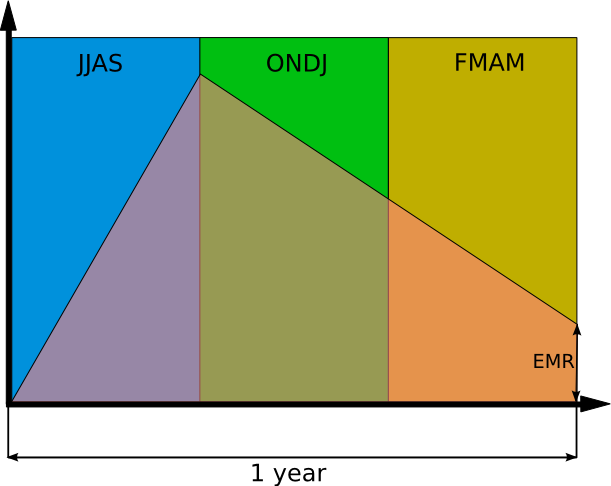
\includegraphics[width=120mm,keepaspectratio=true]{figures/resGrow.png}}
\caption{Figure. Modelled biomass availability through the year.}
\label{fig:resourceGrowing}
\end{figure}


\subsubsection{Agent planning}

Each day the agent will update its knowledge about environment and choose an action to execute (the
decision-making process is defined in the Submodels section 8). The list of available actions is:
\begin{enumerate}
\item Forage - The agent takes multiple walks of a bounded length computed from available
foraging time. Walks are limited to the agent’s Home range. From the visited cells, resource
reward is retrieved based on biomass of the cells. The agent will halt the walk when reward
achieves food needs.
\item Move home - The agent moves from its current home location to a new one within Home
range. The new home settlement is chosen randomly between the dune cells situated in the
richest sectors (containing the highest amount of resources) within Home range. Afterwards, a
Forage Action is executed using half the available daily Foraging time of the agent in order to
include the time spent on movement.
\end{enumerate}


\subsubsection{Adjustment of agent population size}
This processes are executed for each agent:

\begin{enumerate}[1-]
	\item Age. Agent aging (increment human objects age).
	\item Death. Every individual inside an agent will have a probability of dying. At the end of the year
	every individual within an agent must pass two tests to survive:
	\begin{enumerate}
		\item Natural death. Every individual has a 1.5\% annual death probability, except during the
		first four years of life, when this probability is 10\%.
		\item Starvation. Depends on the capability of an agent to fulfil its caloric requirements. Every
		day the agent computes the percentage of needed resources that it was unable to collect.
		This 'starvation value' is accumulated through the year. The cumulative starvation value is
		translated into the overall percentage of full days of the year in which the agent was
		unable to gather sufficient resources. This percentage is translated at the end of the year
		as the probability for the agent to die of starvation.
	\end{enumerate}
	\item Removal. If all the individuals that form an agent are dead, the agent will be removed from
	simulation.
	\item Reproduction. At the end of the year every agent where both adults are still alive will have a
	50\% chance of having a new child.
	\item Emancipation. An agent with individuals coming of age will seek suitable matches among
	agents within its social range. When two individuals coming of age from different agents join a
	new agent is created.
\end{enumerate}

\section{Design concepts}

\subsection{Basic principles}
The behavior defined in this model is derived from the Optimal Foraging Theory (OFT)\cite{Holling1973}, developed
within behavioral ecology and Rational Choice Theory(RCT)\cite{Scott2000} from economics. The main principle of OFT is the maximization of long-term energy gain. In other words, it is usually assumed that animals attempt to maximize the benefit to cost ratio. Evidence exists e.g. among great tits(Parus major), birds that show relatively successful strategies in terms of OFT. Although it is doubtful whether humans attain the optimal rate of energy gain, they do succeed in improving their foraging efficiencies, or 'memorising'. Also, RCT framework backs the decissions of not taking a choice that implies some negative outcome. The term Rational stands for balancing cost of choices in a way that maximizes personal advantage.


\subsection{Emergence}
The model explores the emergence of stable HG populations under different climatic conditions.




%%TODO 
%% afegir la part de comparació amb hard-wired technique vs UCT --> adaptació (BSC day)
\subsection{Adaptation}
At the present moment the model is not interested on the emergence of individual adaptive traits, and
for this reason adaptive options for the agents are limited to the decision making process. The different
agents try to respond to the dynamics of environment choosing Home locations and Foraging actions
depending on their particular situation. The aim is not policy discovering, just adaptative planning.
Adaptive options for the agents are based on the complexity of the decision making process. Actions
costs and outcomes are predefined following the model's configuration, but the order and the use of
them is entirely an agent's choice. Following this reasoning, the different agents will try to adapt the
dynamics of environment (both ecological and social) planning a different set of orders each time step.
\pdfcomment{ATM:future work}A further step in this model will see agents with mixed pool skills that are capable of choosing actions typical of HG and AP populations. Each agent will have different efficiency values for different actions, that will vary in time. In this way, the agent will also adapt specializing its actions.


\subsection{Objectives}
Following the basic principles stated before, the objective for any agent is the survival of its individuals.
This assumption is clearly from optimizing the system, as the different populations won't be guided by
the mission of 'colonizing' the entire landscape. Anyway, this outcome will be seen following
evolutionary mechanisms and positive selection. Well adapted agents will have more possibilities to
survive, thus creating more children and agents with similar cultural traits.

\subsection{Learning}
Foraging learning process is modeled using vertical transmission. A child gradually learns to forage in
an efficient way, and for this reason the available foraging time contributed by children increases until
adulthood.
\subsection{Prediction}
An agent does not keep track of previous rainfall values, so it is not able to predict the future state of
the environment.
\subsection{Sensing \& Information Retrieval from Environment}
An issue seldom addressed in the literature of ABM applications into Social Sciences is the fact that
agents do not have perfect information on their environment. Home range limits the zone that agent
know around its home location. Other issues about bounded rationality is treated in the smart agent section.
 
\subsection{Interaction}
The interaction between agents is currently limited to the \emph{fission} process that is executed when two
agents with adult children are inside social range, and to \emph{information sharing} at the end of the day.


\subsection{Stochasticity}
Stochasticity is used in three different concepts:
\begin{enumerate}
\item Environment. Precipitation is calculated as a estochastical process following a Weibull
distribution.
\item Outcomes. Some actions have different outcomes depending on stochastic processes,
like forage and harvest. It encapsulates the complex process of resources collection (i.e.
risk, variability, etc.), and it is important due to the fact that Actions will be chosen
depending on their outcomes and risk of failure.
\item Life events. Death and reproduction are stochastic processes following realistic
distributions.
\end{enumerate}

\subsection{Collectives}
The agent, atom of the decision-making process, is itself a collective of different related individuals.
\subsection{Observation}
Population dynamics are the most important concepts to derive from the model.

\section{Initialization}
Initial state of the model is divided by entities:

\subsection{Climate}
Rainfall yearly precipitation is a stochastic value calculated from input data, as seen in section 7\pdfcomment{dynamic link}.
Calculated values depend on the initialization seed used in the random number generation, that is
stored as a parameter of the model's configuration. Next parameters can be modified during
initialization time:
	\begin{enumerate}
	\item[EMR] End-of-year minimum residual resources
	\item[AYP] Average Yearly Precipitation
	\item[VYP] Variance in yearly precipitation
	\end{enumerate}


\subsection{Environment}
Ground Model and land features are raster maps created from real data (see also section 7\pdfcomment{symbolic link}). The
model is able to load any raster map with correct values. This process is done during init time from the
file specified in the configuration.


\subsection{Resources}
The conversion functions that create available biomass from landscape and rainfall for each cell use
parameters specified in the configuration. They are based on published research; nevertheless they
can be modified in order to explore different plausible scenarios.

\subsection{Agents}
Several parameters can be changed from the configuration. These values are loaded during init time,
and remain stable during the entire execution. This is the list of parameters used for this model:

\begin{enumerate}
	\item Life-event related:
	\begin{enumerate}
		\item Adulthood age: 15
		\item Dying age (HG/AP): Stochastic distribution %%TODO put a number
		\item Number of agents 
	\end{enumerate}
	\item Resource related:
	\begin{enumerate}
		\item Home Range: 300 cells
		\item Number of sectors: 8
		\item Forage time cost: 30 minutes
		\item Walking Speed: 3 km/hour
	\end{enumerate}
\end{enumerate}


\section{Input data}

\subsection{Rainfall}

Rainfall (yearly precipitation) is the 'environmental engine' of the model. Data for precipitation rate are
extracted from historical data (1871 - 2008). The climate engine is defined as a probability distribution,
from which the total precipitation during a year is derived. The Gamma distribution was the best fit for
the available rainfall dataset. The first approximation was the Weibull distribution. But we wanted to explore
the parameters of mean and stdev in the rain fluctuations to experiment with stressful scenarios and verify
the ressilience of the agents. The characterization of the scenerios was prefigured by the mean and the 
standard deviation of the yearly rain. Weibull distributions are paremeterized with an alpha and a beta 
parameter that would be found with a fit function of the platform R from the historical data we have. The connection
of these parameters with the mean and the standard deviation were not simple formulae in the straight way we wanted. 
The second option, with an excellent match for the shape of our data, was a Gamma distribution\ref{fig:GammaRain}. Again, its parameters alpha and beta are found with a R command. This time, alpha and beta can directly be altered with perturbations derived from the mean and standard deviation explored in the experiments. Table \ref{tab:GammaVSWeibull} a comparison of the relationship of distributions gamma and weibull with the mean and variance parameters.
The function $\Gamma$(Gamma) appearing in the column of weibull distribution has no relationship with ''Gamma'', the statistical distribution. 


	\begin{table}[h]
	\centering
	\begin{tabular}{|l|c||c|}
		\hline
		--		&\emph{Gamma} 		& \emph{Weibull}\\
		\hline
		Mean		&$\alpha/\beta$		& $\lambda\Gamma(1+1/k)$ \\
		\hline
		Variance	&$\alpha/\beta^2$	& $\lambda^2\Gamma(1+2/k)-\mu^2$ \\
		\hline
	\end{tabular}
	\caption{Statistical parameters of Gamma and Weibull distributions.
		$\Gamma(n) = \int^{\infty}_{0} e^{-x}x^{n-1}dx$.    }
	\label{tab:GammaVSWeibull}
	\end{table}

\begin{figure}[h]
\centering
\setlength\fboxsep{0pt}
\setlength\fboxrule{0.5pt}
\fbox{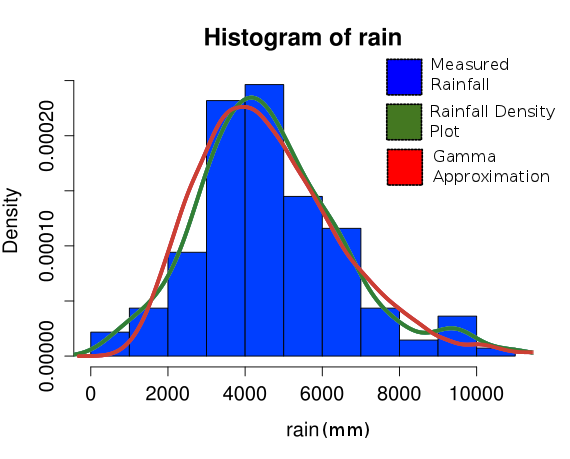
\includegraphics[width=120mm,keepaspectratio=true]{figures/matchRainGamma2.png}}
\caption{Matching of yearly rain distribution shape against gamma distribution shape.}
\label{fig:GammaRain}
\end{figure}


\subsection{Ground Model}
This model is derived from LANDSAT and ASTER satellite imagery (combining pre- and post-monsoon
imagery) and includes DEM and land features. Satellite data are transformed using unsupervised
classification and clustered in the 3 classes (water, interdune and dune). The model is exported as a
Raster map.

\pdfcomment{ATM:future: passarem de 3 categories a 5 de terra. tindrem mes water bodies, rius, etc}


\subsection{Hunter-Gatherer behavior}
Archaeological data are incomplete and limited in terms of derivable behavioural patterns. HG
behaviour for the model was derived from published studies of historical and present-day populations
in similar ecological settings. There are groups of HG that live near N Gujarat (the Van Vargis, see
Nagar 2008). However, these communities have a high degree of interaction with and dependency
from settled agricultural communities for their subsistence strategies. This occurrence constitutes a
strong bias towards the use of these groups to model our HG agents. Instead, we used as surrogates
of our HG population, African groups of the San communities.
Among living and historical HG communities, the San (especially the G/wi and G//ana groups of
Botswana) represent the best-fitting parallel in terms of ecosystem (Tanaka and Sugawara 1996).
These groups are found on a flat plateau in the central part of the Kalahari desert. The landscape
morphology is characterised by fossil rivers and traces of sand dunes. Rainfall is concentrated in the
summer months with c. 400 mm annual average precipitation. The vegetation of the area is dominated
by plants of the Gramineae family (grasses) and a mixture of shrubs of the same genus/families that
are found in North Gujarat.

\pdfcomment{AMT:pg39 : poso la taula de surrogates??? nomes esmentar-los?}

\section{Submodels}

\subsection{Agent execution cycle}



%%TODO
%Smart Agent
	
%	Decision Making :\\
%		stressful environ -> changing rules -> adaptability -> hypoth-deduc
%		we do not have an algebra or HG rules to reason about system dynamic -->
%		--> hypoth-deduc through planning schema --> bandit game --> mdp --> uct
%	Hypoth-Deduct\\
%		Due to the nature of the problem of resource retrieval in the raster lattice we have not
%		developed a logical model to reason about states and actions. We will follow an utility based
%		architecture. The agent has to tackle with resource optimization, large number of uniform 
%		possible cells for exploration and with associated uncertaint. We think it is more reasonable to take an optimization and heuristic search approach
%		instead of a symbolic reasoning based one to synthesize the agent plan. 
%		bandit--->




%	--------MDP\\
%	--------UCT\\
%	--------backed by OptForagTheory & RationalChoiceTheory\\
%	--------BSC day!\\
%	-------- ISSUE { other agents actions are not included in the Hypoth-Deduct schema of
%		-------- UCT. the agents spread over the map more or less uniformly.
%		-------- We do not want competition between them, we want fairplay.
%		-------- We want the group dynamic... Some agent will be lucky, some none.}
%	--------rule agent : we do not want fix set of rules\\
%	----------------learn them? from a setting that we will alter\\
%	----------------to induce change???\\
%	----------------we want adaptability. To the current moment, we choose
%			planning\\


The majority of Agent-Based Models mix knowledge acquisition, decision-making and execution in the
same phase of an agent's execution. This choice is useful if we deal with agents with simple decision-
making processes where the choice of behaviors is predefined. However, this classical approach to
ABM has a major drawback, and is the fact that the agent will have scripted strategies, and for this
reason it won't be able to choose strategies different from the ones defined there.
The model proposed here splits the different phases. During each time step every agent updates its
knowledge about the environment (in the future possibly including other agents)\pdfcomment{ATM: he afegit ``future'' a la frase tot i que a Betesa varem dir que res d'aix\`o}. This action is combined with a set of possible actions, in order to choose which plan of actions will be executed. Several factors can be used to enrich the process:

%%TODO no acabo de pillar tot aquest paragraph. es aixi?


\begin{enumerate}
	\item Agent's goals and agent's preferences referred to the choice of particular actions
	\item The information that the agent perceives from the environment and the reliability of such
	information.
	\item The information collected from other Agents, as well as its reliability.
	\item The feedback the agent receives from engaging into a given activity.
	In this particular model the goal of every agent is to maintain alive its individuals, and the potential
	actions are the ones defined in the document.

%%TODO refine it
 This approach will allow to integrate more sophisticated Artificial Intelligence techniques into the current decision-making process, depending on particular research around this first model.

\end{enumerate}

The execution of the agents during each time step is divided in three different phases:
\begin{enumerate}[1.]
	\item[Knowledge update]
	The agent collects information from the environment, and creates an individual representation of the
	world using its preferences and objectives. Agents will calculate the amount of biomass available in
	each directional sector (utility score), as well as potential settlement zones.
	\item[Action choice]
	The agent decides which actions to execute once knowledge has been collected, based on the
	following steps:
	\begin{enumerate}
		\item Agents checks whether there is any sector inside its home range where resources can be
		obtained. This is calculated based on available foraging time and resources on cells.
		\item If needed resources can be obtained the agent will choose to Forage in one of the Sectors
		where this is possible.
		\item If this is not possible, the agent will choose to Move Home. A collection of possible new homes
		is created based on the quantity of resources inside the Home range from this new location.
		The final location is chosen amongst the ones that fulfill resource requirements.
	\end{enumerate}
	\item[Action]
	After every agent has defined a plan, all of them are executed sequentially following a randomized
	order.
	\item[Information Sharing] 
	Once actions of the day are executed the pipeline proceeds with the information
	sharing phase.
\end{enumerate}


\section{Knowledge}

According to anthropological registers, HGs explore the area around their homes following a excentric direction. Just like a compass divisions, a HG has set of choice directions. Each direction leads to areas where some could be good for foraging and other ones could be poor in resources. Also, anthropological sources describe hunt parties. Sometimes males of the familiar groups join in a group of hunters and spend several days apart from the home hunting in the whereabouts of the home range. This first stage of our models is not considering yet agent coordination and cooperation, so we stick to simple hunt actions with one hunter (and grown children) with a few hours duration, which
are subsumed under ForageAction.
 
We decided to endow agents with a map of cells of the world bounded by their home range. The circled area by the home range is divided in equal slices called sectors. The number of sectors is parameterizable though a configuration file.   
For each sector their cells are stored and an utility scoring is assigned. For foraging decissions the utility is the sum of resources of the cells that compose it and for the MoveHome action the utility is %TODO

Each time step the amount of resources in each cell changes due to the growing dynamics of biomass and to the possible foraging practices of other agents. The updating of utilities must be done each time step. The default update of utilities is omniscient inside the home range. The agent acces directly to all the information inside the area of its home range, outside of it the agent does not map more cells. We assume the agent can read the last updated value in resources for any cell concerning the update procedure. 

At this stage the agent does not stores knowledge about the other agents.

\subsection{Low Ressolution map}

In our experiments agents have been working with two different engines for decision making. The planning engine produces millions of acces to the cell storages in the search of profitable traces of actions. Each state in the search tree requires updates and many calculi managing the cells in the sector visited by the action. 
This represents around 40,000 cells per sector to manage for a home range with a radius of 300 cells. Supporting this amount of information and accesses in a simulation with 100 agents implied traces that lasted more than eight hours of computation per year simulated. This is not affordable for the scales we need to simulate. Some real world cultural transitions last about the order of hundreds of years. The direction taken to reduce the load of the planning synthesis was to reduce the resolution of the representation of the world in the mind of the agent. Indeed real HGs when think about profitable patches in his domains do not have a high ressolution representation of the resources. They have fuzzy mind maps of more or less large rich areas. They do not think with a granularity of few meters when planning the day. 
They think about patches that would cover several high resolution cells of our model.

Each agent has private lists of references to low ressolution cells, sectors. The low resolution cells belong to a shared raster. Each low resolution cell covers an area of 60x60 high resolution cells. Each time step, once the high resolution raster world receives all the updates, the utility of the low resolution cells and minds(sectors) of the agents is updated \ref{figLRRepr}.

		\begin{figure}[!h]
		\centering
		\setlength\fboxsep{0pt}
		\setlength\fboxrule{0.5pt}
		\fbox{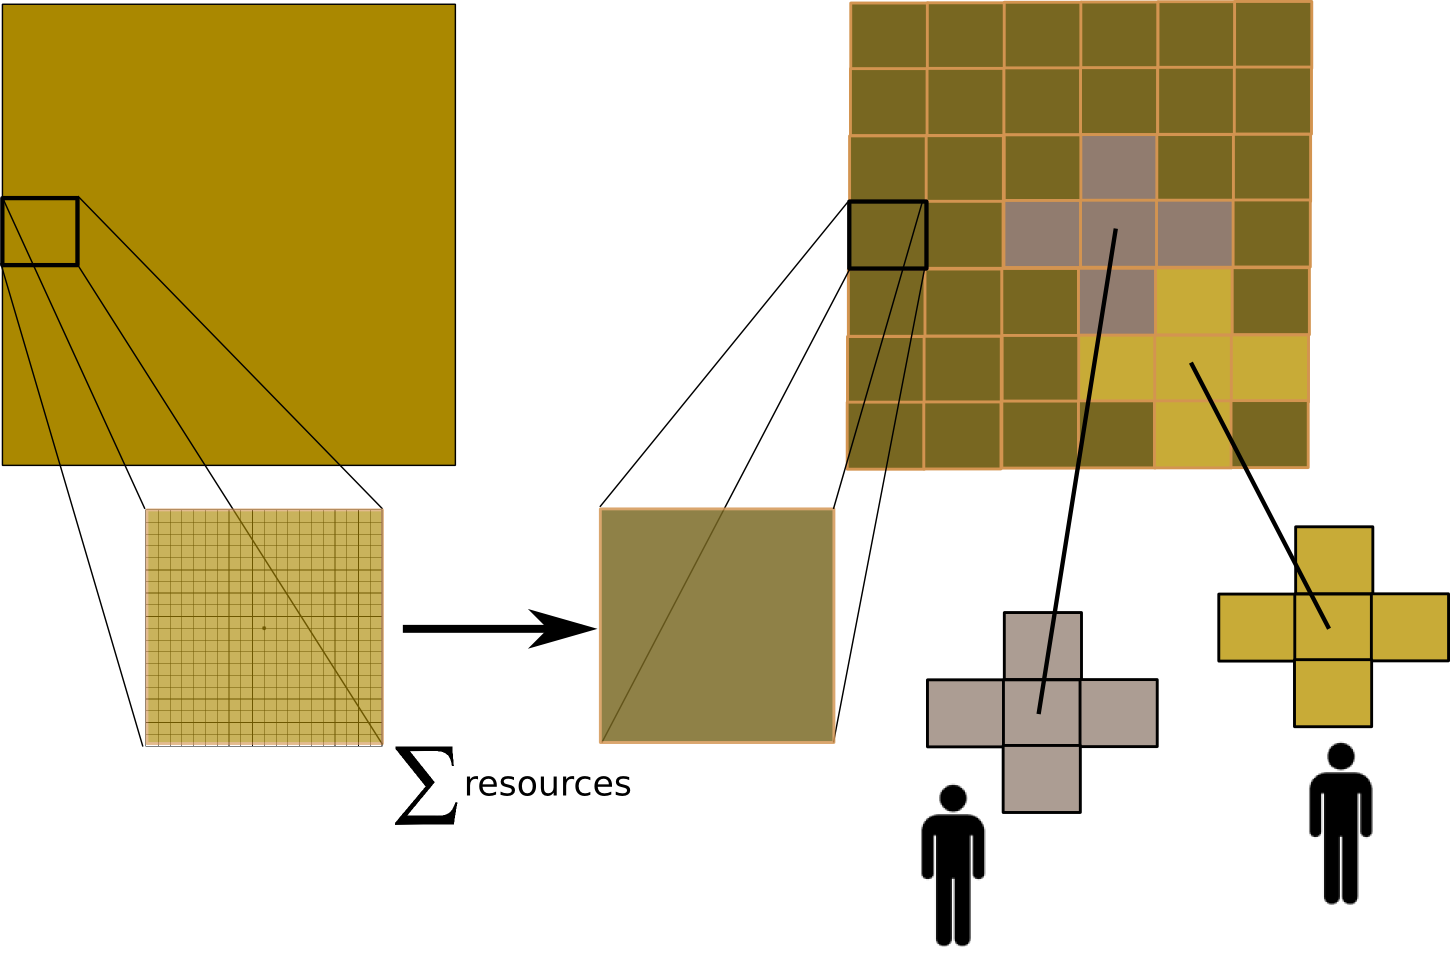
\includegraphics[width=80mm,keepaspectratio=true]{figures/LRmaps1.png}}
		\caption{HR vs LR correspondence}
		\label{fig:LRMaps1}
		\end{figure}


Extrapolation and integer division are used to translate coordinates from low resolution to high resolution. 

The utility of a low resolution cell is the sum of resources of the covered cells. Now the sectors in the mind of the agent contain less items. When the planning engine simulates the effect of actions processes a low resolution cell iterating over a formula to emulate the steps the agent would do visiting the high resolution cells.      



\subsection{Partial Information}

parla del partial mind


\subsection{Information Sharing}

Information sharing and knowledge exchange is a crutial activity for performance enhancing on everyday challenges. In our study of resilience of social groups in arid environments we try to explain the conditions that trigger or inhibite the change of social groups moving from hunting strategies to agropastoralist strategies. The most successful strategies will be passed between agents of our simulation in a cultural transmission modelized framework. Our first results are based on sharing environmental information concerning resource allocation in the environment. Our simulations show that simulating individuals with partial information of the environment, but sharing it with other
neighbour agents, allows them to achieve a resource retrieval as good as if they would be endowed with complete perfect information of the resource allocation.

We have developed an agent based model to study the resilience of hunter-gatherer groups and agropastoralists groups in the edge of agriculture spreading(12000 BP). The aim is to study the environmental conditions that favor one group versus the other applying the dynamics of coevolution and movility of agent's strategies. The evolutive pression of the environment selects the social group according to the succes in resource retrieval. Each agent has a pack of skills to solve the problem of resource threshold for survival. The proficiency of these skills accounts as shareable knowledge that other agents can copy or learn. An agent will gain or loose proficiency based on the rate of use of some skills instead of the others. The dynamics of forgetting and learning will induce profiles of patterns of competence. The profiles are correlated with the dynamic of the environment. It will allow to discover if
conditions favour one concrete group, or maybe favour a mix of strategies or a periodical change from one profile to another.

We consider the introduction of social networks as an important factor for ressilience as it acts as a safety network for unlucky agents affected by detrimental variabilty of environment conditions. A social network will be a source of help in the form of resources, environmental information and transmission of knowledge for survival strategies.

Three experiments have been launched to compare three kind of mind models for hunter gatherer agents. Each experiment simulates one kind of mind model. For the first experiment the agents had complete and updated information of the amount of resources around their settlement in a fixed distance radius estimated from anthropological observations. The second experiment considered agents that had partial information consisting in statistical guessings and real information gathered when a terrain patch was explicit visited for hunting or foraging. The third experiment simulated agents that lived with partial information like the ones from experiment number two but with the addition of sharing of information pieces from their knowledge bank. The results confirm that information sharing increases resilience under conditions where partial information and uncertainty is taken into account as a phenomenon to model. It puts the next milestone to include more social actions and the modelization of cultural transmission.



\section{Decision Making}

bandits
MDP
UCT


\begin{figure}[h]
\centering
\setlength\fboxsep{0pt}
\setlength\fboxrule{0.5pt}
\fbox{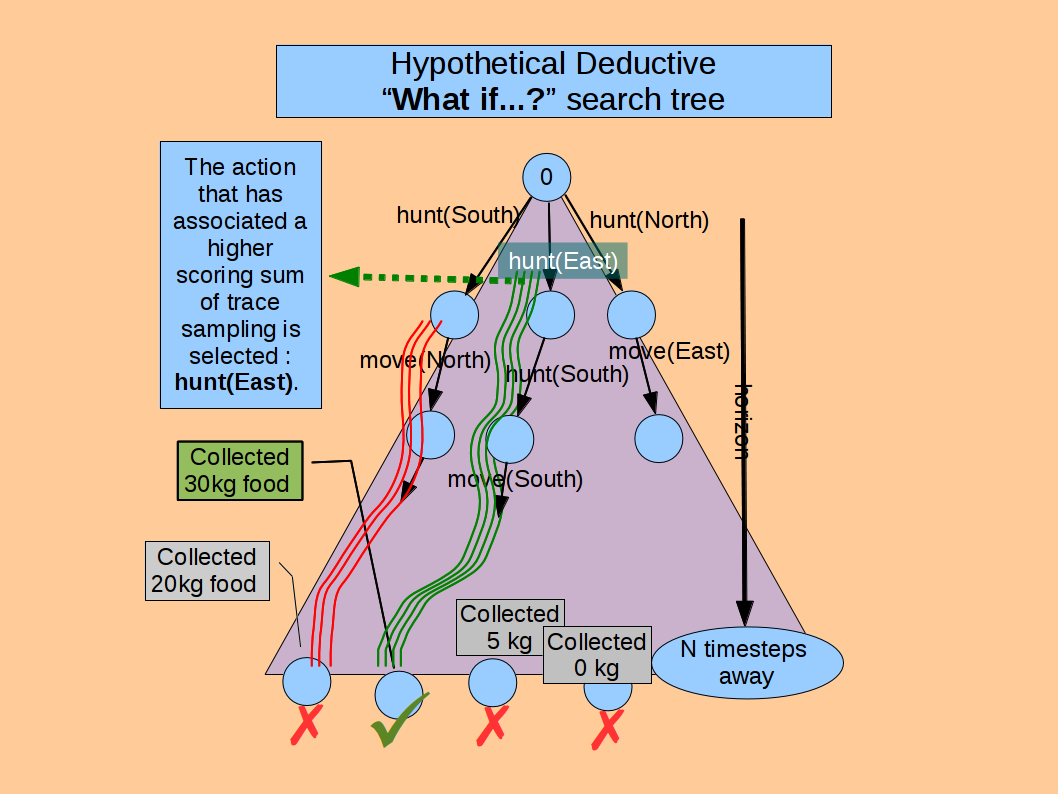
\includegraphics[width=150mm,keepaspectratio=true]{figures/uctTree.png}}
\caption{Figure. Uct search tree.}
\label{fig:uctTree}
\end{figure}


performance
LR
MDPState reference
Extrapolation


%%%%%%%%%%%%%%%%%%%%%%%%%%%%%%%%%%%%%%%%%%%%%%%%%%%%%%%%%%%%%%%
\chapter{Annex 1}

%TODO diagrames de classes

\chapter {Annex 2}

%TODO elicitation procedures : ECOTONO,meetings,interviews,simulpast seminars (other CSx give opinion)

%%%%%%%%%%%%%%%%%%%%%%%%%%%%%%%%%%%%%%%%%%%%%%%%%%%%%%%%%%%%%%%

\chapter{Bibliography}
\begin{thebibliography}{49}

\bibitem{Epstein1999} 
	J.M. Epstein. 
	\emph{Agent-based computational models and generative social science. Generative Social
	Science: Studies in Agent-Based Computational Modelling}, pages 4-46
	1999

\bibitem{EpsteinAxtell}
	J.M. Epstein and R. Axtell.
	\emph{Growing Artificial Societies}, 1996.
	1996

\bibitem{Epstein2008}
	Joshua Epstein
	\emph{Why Model?}.
	2008.

\bibitem{Axelrod2003}
	R. Axelrod. 
	\emph{Advancing the Art of Simulation in the Social Sciences. Japanese Journal for Management Information System, Special Issue on Agent-Based Modelling}, Vol. 12, No. 3 
	Dec. 2003. 

\bibitem{Axelrod2007}
	R. Axelrod. 
	\emph{Simulation in Social Sciences. Handbook of research on nature-inspired computing for economics and management}, 1:90, 
	2007

\bibitem{JDoran}
	Doran, J., 
	\emph{Prospects for Agent-Based modelling in Archaeology}. Archeologia e Calcolatori, 10, 33-44.
	1999

\bibitem{RussellNorvig}
	Stuart Russell and Peter Norvig.
	\emph{Artificial Intelligence: A Modern Approach} 3rd edition.
	2009

\bibitem{GilbertABM}
	Nigel Gilbert.
	\emph{Agent-Based Models}. SAGE Publications, California.
	2008

\bibitem{GilbertArtfSoc}
	Nigel Gilbert, Rosaria Conte.
	\emph{Artificial Societies. The computer simulation of social life}.
	1995.

\bibitem{TaberAndTimpone1996}
	Charles S. Taber, Richard J. Timpone.
	\emph{Computational modelling}.
	1996.

\bibitem{GilbertTroitzsch}
	Gilbert, N., Troitzsch, K.G.,
	\emph{Simulation for the Social Scientist}. Open University Press, USA.
	2008.

\bibitem{Scott2000}
	John Scott
	\emph{Rational Choice Theory}. From Understanding Contemporary Society: Theories of The Present, edited by G. Browning,
	A. Halcli, and F. Webster. (Sage Publications, 2000).
	2000.

\bibitem{Wooldridge2002}
	Michael Wooldridge.
	\emph{An Introduction to Multiagent Systems}
	2002

\bibitem{WooldridgeJennings1995}
	 Michael Wooldridge, Nick Jennings.
	\emph{Intelligent Agents: Theory and Practice}  Knowledge Engineering Review Volume 10 No 2. (c) Cambridge
	University Press 
	1995

\bibitem{Wooldridge1997}
	 Michael Wooldridge.
	\emph{Agent-based software engineering}, IEE Proc. Software Engineering 144 (1) 
	1997.

\bibitem{Shoham1990}
	Yoav Shoham.
	\emph{Agent-Oriented Programming. Stanford University: Computer Science Department.(Technical Report STAN-CS-90-1335).}
	1990 

\bibitem{Lake}
	Lake, M W,
	\emph{2000. Computer Simulation of Mesolithic Foraging, in: Gumerman, G. J., Kohler, T.A. (Eds.), Dynamics in Human and Primate Societies: Agent-Based Modelling of Social and Spatial Processes}, Oxford University Press, New York, pp. 107-143.
\bibitem{Sugarscape}
	Sugarscape.
	\emph{http://ccl.northwestern.edu/netlogo/models/community/Sugarscape}

\bibitem{Pavon2008}
	Juan Pavón, Millán Arroyo, Samer Hassan, Candelaria Sansores.
	\emph{Agent-based modelling and simulation for the analysis of social patterns}. Pattern Recognition Letters 29(8): 1039-1048 
	2008

%\bibitem{Pidd2012}
%	Pidd
%	\emph{Pidd book}.
%	2012.
%\bibitem{Pidd2010}
%	Pidd
%	\emph{Pidd book}.
%	2010.
\bibitem{Pidd2003}
	Mike Pidd.
	\emph{Tools for Thinking: Modelling in Management Science, 2nd Ed. Wiley.Chichester,UK}.
	2003.

\bibitem{Robinson2008}
	Kathy Kotiadis, Stewart Robinson
	\emph{CONCEPTUAL MODELLING: KNOWLEDGE ACQUISITION AND MODEL ABSTRACTION}.
	2008.

\bibitem{GrimmBergerODD2012}
	Grimm V, Berger U, DeAngelis D L, Polhill J G, Giske J and Railsback S F 
	\emph{The ODD protocol: A review and first update}. 
	Ecological Modelling 221 (23), 2760-2768.
	2010. 
	

\bibitem{McGivernAndRueger}
	Patrick McGivern, University of Wollongong.
	Alexander Rueger, University of Alberta.
	\emph{Hierarchies and levels of reality}.
	2010.

\bibitem{Unity_of_Science}
	\emph{The Unity of Science}, Stanford Encyclopedia of Philosophy 
	(http://plato.stanford.edu/entries/scientific-unity/).
	2007.

\bibitem{Premo2010}
	L.S.Premo
	Equifinality and Explanation:The Role of Agent-Based Modeling in Postpositivist Archeology, 
	published at Simulating Change; archeology into the twenty-first century Ed. Andre Costopoulos, Mark Lake.
	2012.

\bibitem{Peirce_Abduction}
	Peirce, C. S. 
	Abduction (cf. Hypothesis [as a form of reasoning], Retroduction, Presumption [as a form of reasoning], À posteriori Reasoning ). Commens Dictionary of Peirce's Terms.
	
\bibitem{PerezAndBatten2006}
	Pascal Perez and David Batten
	\emph{Complex Science for a Complex World; Exploring Human Ecosystems with Agents}. 
	August 2006.

\bibitem{Box1979}
	George Box 
	Section heading, page 2 of Box's paper, 
	\emph{Robustness in the Strategy of Scientific Model Building} in Robustness in Statistics: Proceedings of a Workshop (1979) 
	edited by RL Launer and GN Wilkinson
	May 1979.

\bibitem{MWilliams1999}
	Malcolm Williams
	\emph{Science and Social Science: An Introduction.} Psychology Press 
	1999. 

\bibitem{GordonBurt2010}
	Gordon Burt
	\emph{Conflict, Complexity and Mathematical Social Science}
	2010.

\bibitem{Coleman1964}
	Coleman,J.S.
	\emph{An introduction to mathematical sociology}. New York: Free Press.
	1964.

\bibitem{Balci1988}
	Balci
	\emph{Balci book}.
	1988.

\bibitem{Heath2009}
	Heath
	\emph{Heath book}.
	2009.

\bibitem{Banks1998}
	Banks
	\emph{Banks book}.
	1998.

\bibitem{Davies2003}
	Davies
	\emph{Davies book}.
	2003.

\bibitem{Axelrod1997a}
	Axelrod
	\emph{Axelrod book}.
	1997.


\bibitem{Bonabeau2002}
	Eric Bonabeau
	\emph{Agent-based modelling: Methods and techniques for simulating human systems, PNAS, vol 99} 
	2002.

\bibitem{Axtell2000}
	Robert L. Axtell
	\emph{WHY AGENTS? ON THE VARIED MOTIVATIONS FOR AGENT COMPUTING IN THE SOCIAL SCIENCES.The Brookings Institution}
	2000.

\bibitem{Helbing2000}
	D. Helbing, I. Farkas, and T. Vicsek 
	\emph{Simulating dynamical features of escape panic. Nature 407, pg 487-490.}
	2000.

\bibitem{MelanieMitchell2009}
	Melanie Mitchell
	\emph{Complexity, a Guided Tour.}
	2009.

\bibitem{Holland1997}
	John Holland
	\emph{Philosophica 59 (1997, 1) pp. 11-40. Emergence.}
	1997.

\bibitem{MillerPage2007}
	John H. Miller, Scott E. Page
	\emph{Complex Adaptive Systems: An Introduction to Computational Models of Social Life (Princeton Studies in Complexity)}
	2007.

\bibitem{Vicsek2002}
	Tamas Vicsek
	\emph{Complexity. The bigger picture. Nature 418, pg 131.}
	2002.	


\bibitem{TakahashiSallachRouchier2007}
	Takahashi, Shingo; Sallach, David; Rouchier, Juliette
	\emph{Advancing Social Simulation: The First World Congress, Springer, p. 354, ISBN 978-4-431-73150-4}.
	2007.

\bibitem{Gross2008}
	Claudius Gross
	\emph{Complex and Adaptive Dynamical Systems.}
	2008.

\bibitem{Holling1973}
	Holling CS 
	\emph{Resilience and Stability of Ecological Systems Annual Review of Ecology and Systematics} Vol. 4: 1-23.
	1973. 

	
\bibitem{Dawkins1990}
	Richard Dawkins
	\emph{The Selfish Gene.Oxford University Press, 2nd edition}	
	1990.

\bibitem{Stanford_CultEvol}
	Tim Lewens
	\emph{"Cultural Evolution", The Stanford Encyclopedia of Philosophy}. 
	(Spring 2013 Edition), Edward N. Zalta (ed.), 
	URL = <http://plato.stanford.edu/archives/spr2013/entries/evolution-cultural/>. 
	2013.

\bibitem{hysteresisDef}
	Mielke, A. and Roubicek, T.. 
	\emph{"A Rate-Independent Model for Inelastic Behavior of Shape-Memory Alloys"}. 
	Multiscale Model. Simul. 1 (4). 
	2003.

\end{thebibliography}

\end{document}
